%%%%%%%%%%%%%%%%%%%%%%%%%%%%%%%%%%%%%%%%%%  不使用 authblk 包制作标题  %%%%%%%%%%%%%%%%%%%%%%%%%%%%%%%%%%%%%%%%%%%%%%
%-------------------------------PPT Title-------------------------------------
\title{AI~For~Science:\\知识图谱在化学-化工领域的应用}
%-----------------------------------------------------------------------------

%----------------------------Author & Date------------------------------------
%\author[\textrm{Jun\_Jiang}]{姜\;\;骏\inst{}} %[]{} (optional, use only with lots of authors)
%% - Give the names in the same order as the appear in the paper.
%% - Use the \inst{?} command only if the authors have different
%%   affiliation.
\institute[BCC]{\inst{}%
%\institute[Gain~Strong]{\inst{}%
\vskip 2pt 中科合成油技术有限公司\\
\vskip 3pt 北京市计算中心}
%云平台事业部~材料计算团队}
%\vskip -20pt {\large 格致斯创~科技}}
\date[\today] % (optional, should be abbreviation of conference name)
{	%{\fontsize{6.2pt}{4.2pt}\selectfont{\textcolor{blue}{E-mail:~}\url{jiangjun@bcc.ac.cn}}}
\vskip 15 pt {\fontsize{8.2pt}{6.2pt}\selectfont{%清华大学\;\;物理系% 报告地点
	\vskip 5 pt \textrm{2025.01}}}
}

%% - Either use conference name or its abbreviation
%% - Not really information to the audience, more for people (including
%%   yourself) who are reading the slides onlin%%   yourself) who are reading the slides onlin%%   yourself) who are reading the slides onlineee
%%%%%%%%%%%%%%%%%%%%%%%%%%%%%%%%%%%%%%%%%%%%%%%%%%%%%%%%%%%%%%%%%%%%%%%%%%%%%%%%%%%%%%%%%%%%%%%%%%%%%%%%%%%%%%%%%%%%%

\subject{}
% This is only inserted into the PDF information catalog. Can be left
% out.
%\maketitle
\frame
{
%	\frametitle{\fontsize{9.5pt}{5.2pt}\selectfont{\textcolor{orange}{“大数据中心调研座谈会”}}}
\titlepage
}
%-----------------------------------------------------------------------------

%------------------------------------------------------------------------------列出全文 outline ---------------------------------------------------------------------------------
\section*{}
\frame[allowframebreaks]
{
  \frametitle{Outline}
%  \frametitle{\textcolor{mycolor}{\secname}}
  \tableofcontents%[current,currentsection,currentsubsection]
}
%在每个section之前列出全部Outline
%类似的在每个subsection之前列出全部Outline是\AtBeginSubsection[]
%\AtBeginSection[]
%{
%  \frame<handout:0>%[allowframebreaks]
%  {
%    \frametitle{Outline}
%%全部Outline中,本部分加亮
%    \tableofcontents[current,currentsection]
%  }
%}

%-----------------------------------------------PPT main Body------------------------------------------------------------------------------------
\small
\begin{frame}{科学研究的重要助手:~计算模拟}
\begin{figure}[h!]
\vspace*{-0.18in}
\centering
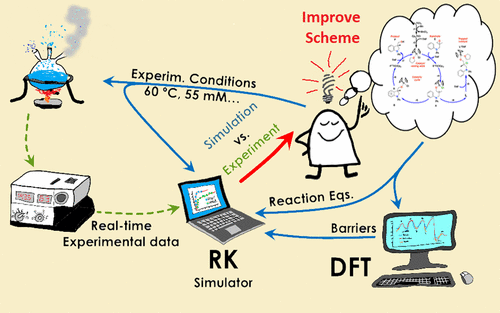
\includegraphics[height=2.55in,width=4.05in]{Figures/Schematic_Material-Design.png}
%\caption{\tiny \textrm{Pseudopotential for metallic sodium, based on the empty core model and screened by the Thomas-Fermi dielectric function.}}%(与文献\cite{EPJB33-47_2003}图1对比)
%\caption{\tiny \textrm{Pseudopotential for metallic sodium, based on the empty core model and screened by the Thomas-Fermi dielectric function.}}%(与文献\cite{EPJB33-47_2003}图1对比)
\label{Schematic_Material-Design}
\end{figure}
\end{frame}

%\frame
%{
%	\frametitle{材料模拟的基本思想和方法}
%\begin{figure}[h!]
%\vspace*{-0.25in}
%\centering
%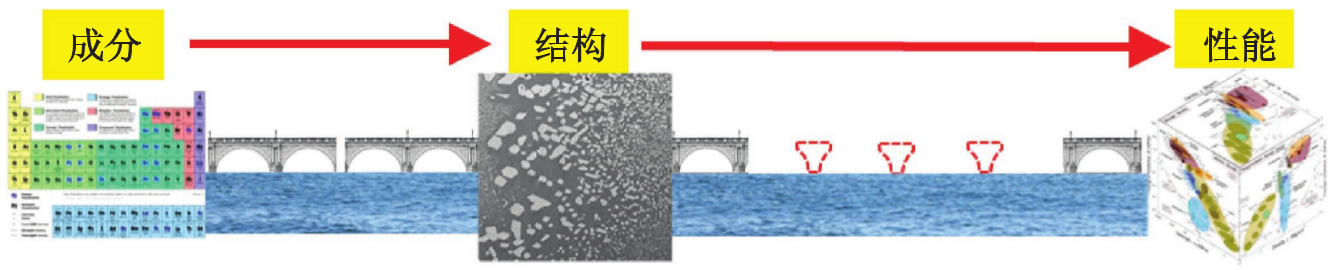
\includegraphics[height=0.80in,width=4.05in]{Figures/MGE-2.png}
%%\caption{\tiny \textrm{Pseudopotential for metallic sodium, based on the empty core model and screened by the Thomas-Fermi dielectric function.}}%(与文献\cite{EPJB33-47_2003}图1对比)
%\label{MGE}
%\end{figure}
%\begin{minipage}[c]{0.30\textwidth}
%\begin{itemize}%[+-| alert@+>]
%\vspace*{-2.25in}
% {\fontsize{7.5pt}{6.0pt}\selectfont
%	 \setlength{\itemsep}{10pt}
% \item 变革研发模式,计算-实验-理论-数据科学相融合: 高效、低耗按需设计
% \item 数据驱动的材料创新平台主要面向复杂材料的模拟}
% \end{itemize}
%\end{minipage}
%\hfill
%\begin{minipage}[b]{0.68\textwidth}
%\begin{figure}[h!]
%%\vspace*{-0.25in}
%\centering
%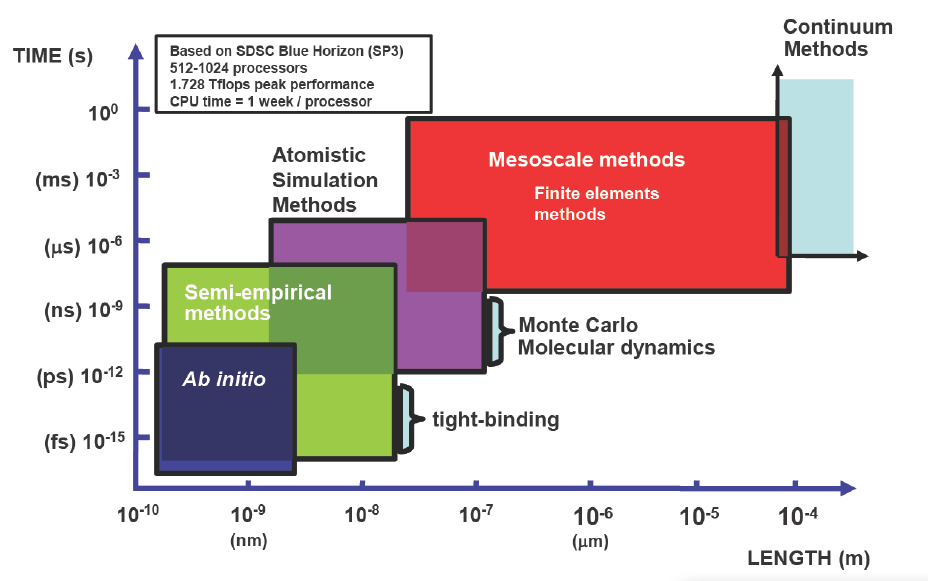
\includegraphics[height=1.80in,width=2.75in]{Figures/Multi-Scale-6.png}
%%\caption{\tiny \textrm{Pseudopotential for metallic sodium, based on the empty core model and screened by the Thomas-Fermi dielectric function.}}%(与文献\cite{EPJB33-47_2003}图1对比)
%\label{Multi-Scale}
%\end{figure}
%\end{minipage}
%}
%
%\frame
%{
%	\frametitle{科学研究的范式变更}
%\begin{figure}[h!]
%\vspace*{-0.28in}
%\centering
%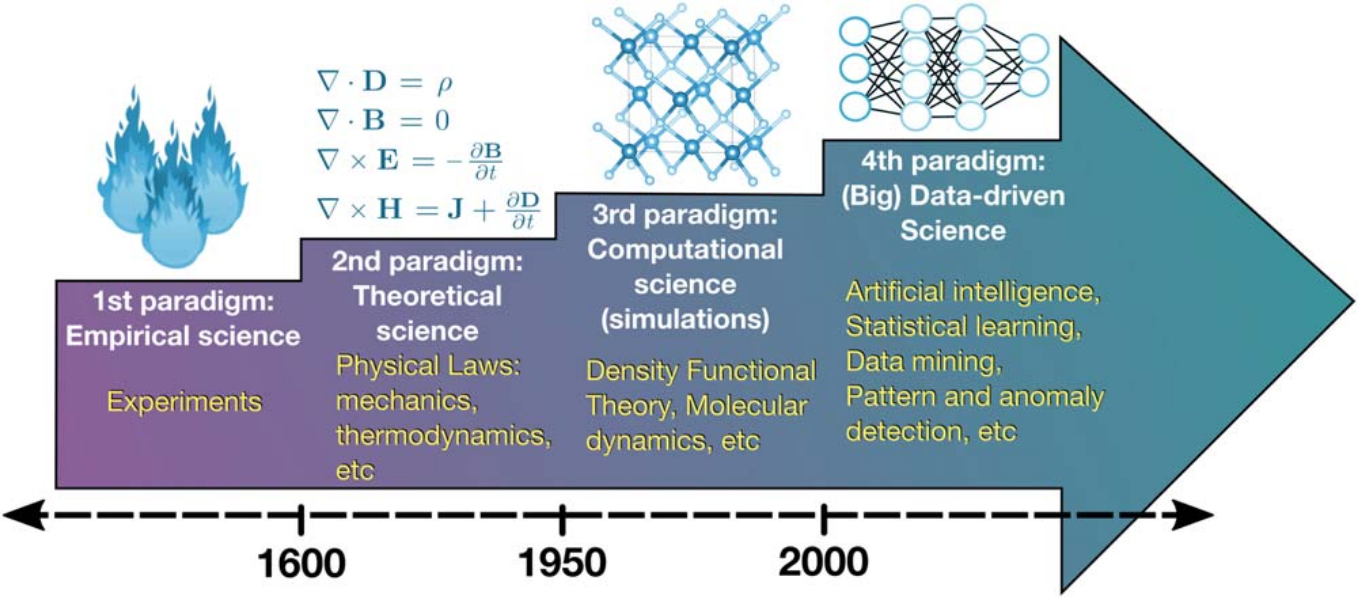
\includegraphics[height=2.00in,width=4.15in]{Figures/Four_Model_3.png}
%%\caption{\tiny \textrm{Pseudopotential for metallic sodium, based on the empty core model and screened by the Thomas-Fermi dielectric function.}}%(与文献\cite{EPJB33-47_2003}图1对比)
%\label{Four_Model}
%\end{figure}
%\begin{minipage}[b]{0.48\textwidth}
% {\fontsize{7.5pt}{6.0pt}\selectfont\begin{itemize}%[+-| alert@+>]
%	 \setlength{\itemsep}{10pt}
% \item 逐步趋于理性
% \item 逐步趋于复杂
% \end{itemize}}
%\end{minipage}
%\hfill
%\begin{minipage}[b]{0.48\textwidth}
% {\fontsize{7.5pt}{6.0pt}\selectfont\begin{itemize}%[+-| alert@+>]
%	 \setlength{\itemsep}{10pt}
% \item 逐步趋于抽象
% \item 逐步趋于深刻
% \end{itemize}}
%\end{minipage}
%}
%
%\frame
%{
%	\frametitle{数据驱动的科学研究}
%前所未有的计算能力和大规模的数据收集能力%,现代科学正在进入“第四范式”:
%\begin{figure}[h!]
%%\vspace*{-0.05in}
%\centering
%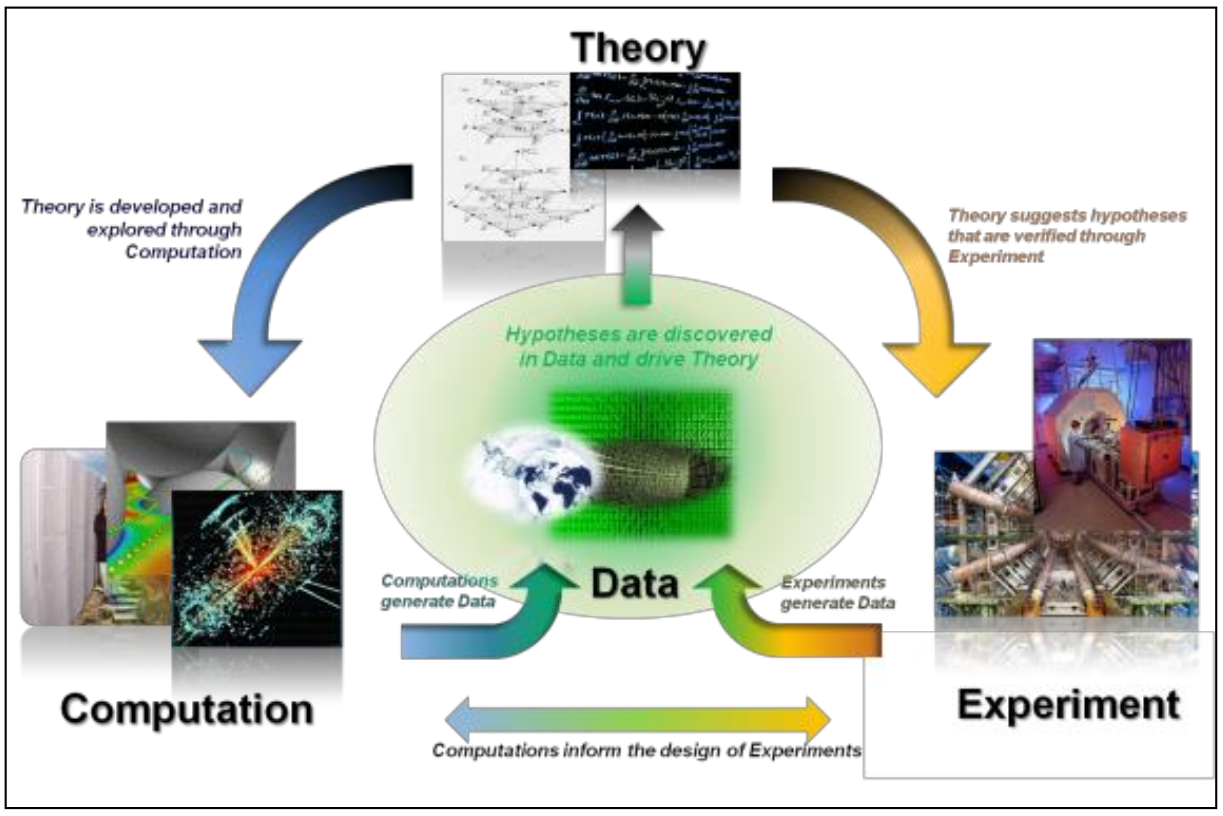
\includegraphics[height=2.30in,width=3.70in]{Figures/Four_Model_1.png}
%%\caption{\tiny \textrm{Pseudopotential for metallic sodium, based on the empty core model and screened by the Thomas-Fermi dielectric function.}}%(与文献\cite{EPJB33-47_2003}图1对比)
%\label{Four_Model_1}
%\end{figure}
%科学的新驱动力:~\textcolor{red}{密集数据}+\textcolor{red}{人工智能}\\
%}
%
\frame
{
	\frametitle{数据、信息与知识}
\begin{figure}[h!]
\centering
\vskip -10pt
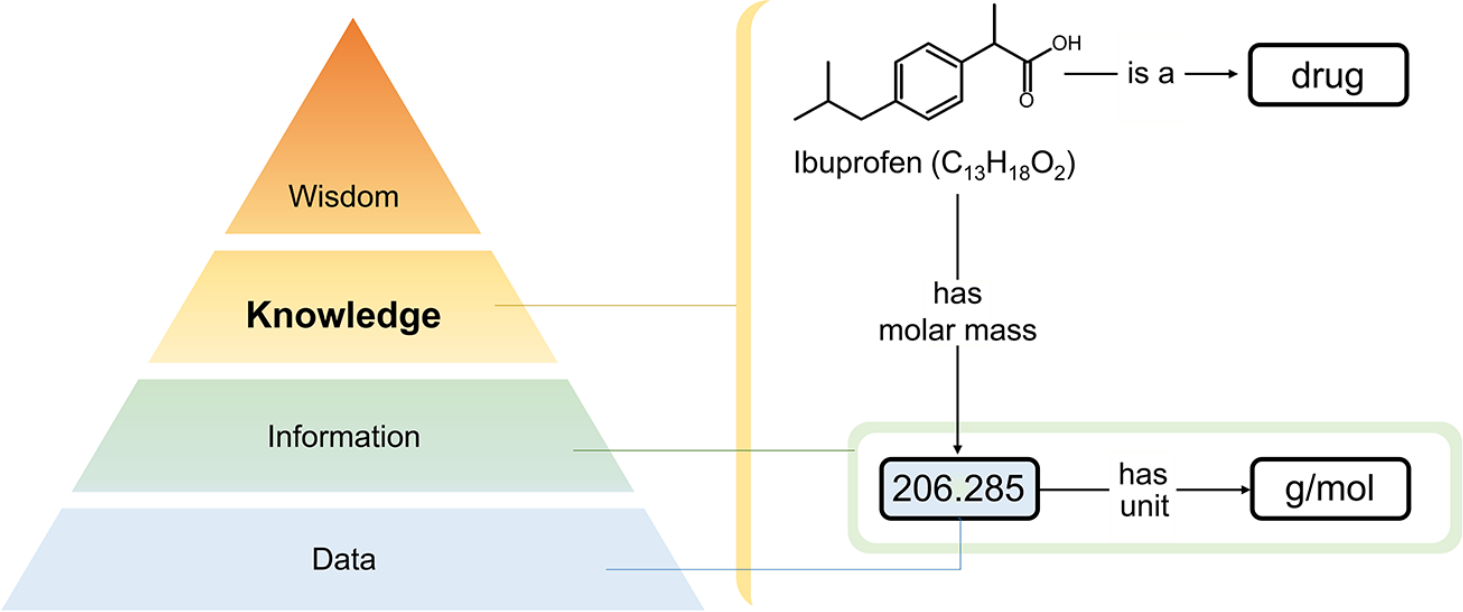
\includegraphics[height=1.75in,width=4.00in,viewport=0 0 1490 615,clip]{Figures/DIKW_pyramid-illustrating-data_information-knowledge.png}
\caption{\tiny\textrm{Schematic representation of the DIKW pyramid illustrating the meaning of data, inforamation, and knowledge in the chemical context.\cite{ACR56-128_2023}}}%(与文献\cite{EPJB33-47_2003}图1对比)
\label{Fig:Knowledge-based_system}
\end{figure}
\textcolor{magenta}{知识}\textrm{(Knowledge)}:\\
哲学学科——诸如认知论和方法论——中的核心主题
}

\section{化学-化工类知识图谱}
\subsection{知识图谱基础知识}
\frame
{
	\frametitle{知识图谱}
	\textcolor{blue}{知识图谱}~\textrm{(Knowledge Graph)}:
	\begin{itemize}
		\item 一种用于组织、表示和存储知识的图形化数据结构形式
		\item \textcolor{purple}{目的}:~使计算机能够更好地认知、理解和推理知识\\
			仿照人类对于知识的认知、理解方式将实体\textrm{(Entities)}、关系\textrm{(Relationship)}和属性\textrm{(Attributes)}以图形的形式呈现出来,
		\item \textcolor{purple}{技术底层}:~基于语义网\textrm{(Semantic Web)}技术\\
			以\textrm{Web}数据的内容(即语义)为核心,用机器能够理解和处理的方式链接起来的海量分布式数据库
	\end{itemize}
%	知识图谱得益于\textrm{Web}的发展(主要的是数据层面),有着来源于\textrm{KR}、\textrm{NLP}、\textrm{Web}、\textrm{AI}多个方面的基因
\begin{figure}[h!]
\centering
\vskip -8pt
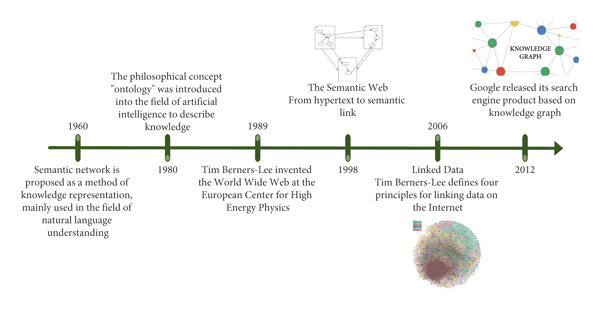
\includegraphics[height=1.00in,width=2.50in,viewport=0 0 160 75,clip]{Figures/Development-history-of-the-knowledge-graph.jpg}
\caption{\tiny\textrm{Schematic representation of the development history of the Knowledge Graph.}}%(与文献\cite{EPJB33-47_2003}图1对比)
\label{Fig:Knowledge-history}
\end{figure}
}

\frame
{
	\frametitle{知识图谱的要素}
知识图谱以图形结构的方式,通常使用节点(实体)和连线/边(关系)的形式表示知识\\
%这种结构使得知识点之间的关联关系更加清晰和可视化
%
%主要的关键词为:
\begin{itemize}
	\item {\fontsize{7.2pt}{5.2pt}\selectfont{实体\textrm{(Entities)}:~知识图谱中的实体是指具体的事物、概念、人物、地点等,每个实体都有一个唯一的标识符}}\\
		{\fontsize{6.2pt}{5.2pt}\selectfont{例如,在化学知识图谱中,分子、合成体、密度等都是实体}}
	\item {\fontsize{7.2pt}{5.2pt}\selectfont{关系\textrm{(Relationships)}:~实体之间的关系表示不同实体之间的连接或互动。这些关系可以是有向的或无向的,用于描述实体之间的各种联系}}\\
		{\fontsize{6.2pt}{5.2pt}\selectfont{如” 具有”、” 属于”、”值为” 等}}
	\item {\fontsize{7.2pt}{5.2pt}\selectfont{属性\textrm{(Attributes)}:~实体可以有一些描述性的属性,这些属性是实体相关的额外信息}}\\
		{\fontsize{6.2pt}{5.2pt}\selectfont{例如,分子(实体)的属性,包括分子量、化合价、密度等}}
\end{itemize}
\begin{figure}[h!]
\centering
\vskip -8pt
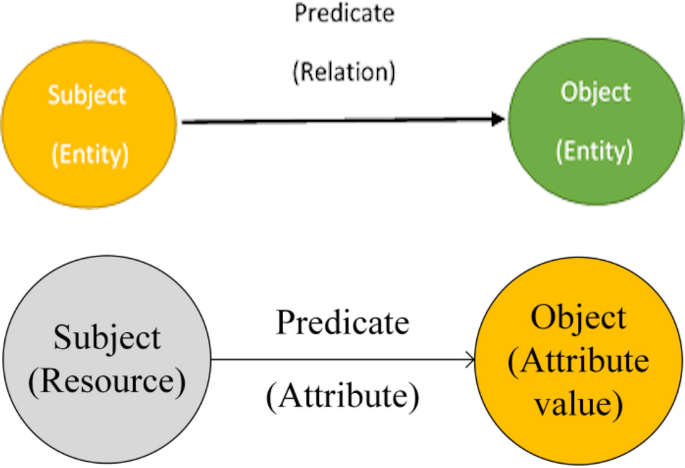
\includegraphics[height=1.05in,width=1.50in,viewport=0 0 690 470,clip]{Figures/KG-Entity-relation_0.png}
\caption{\tiny\textrm{Schematic representation of the relationship between entites.}}%(与文献\cite{EPJB33-47_2003}图1对比)
\label{Fig:KG-Entity-relations}
\end{figure}
}

\subsection{国外的化学-化工知识图谱的建设现状与目标}
\frame
{
	\frametitle{知识图谱的起点:~化学物种的描述}
		\textrm{OntoSpecites}:~主要纪录化学物种的知识,包括分子式、电荷、分子量和自旋多重度等
\begin{figure}[h!]
\centering
\vskip -1pt
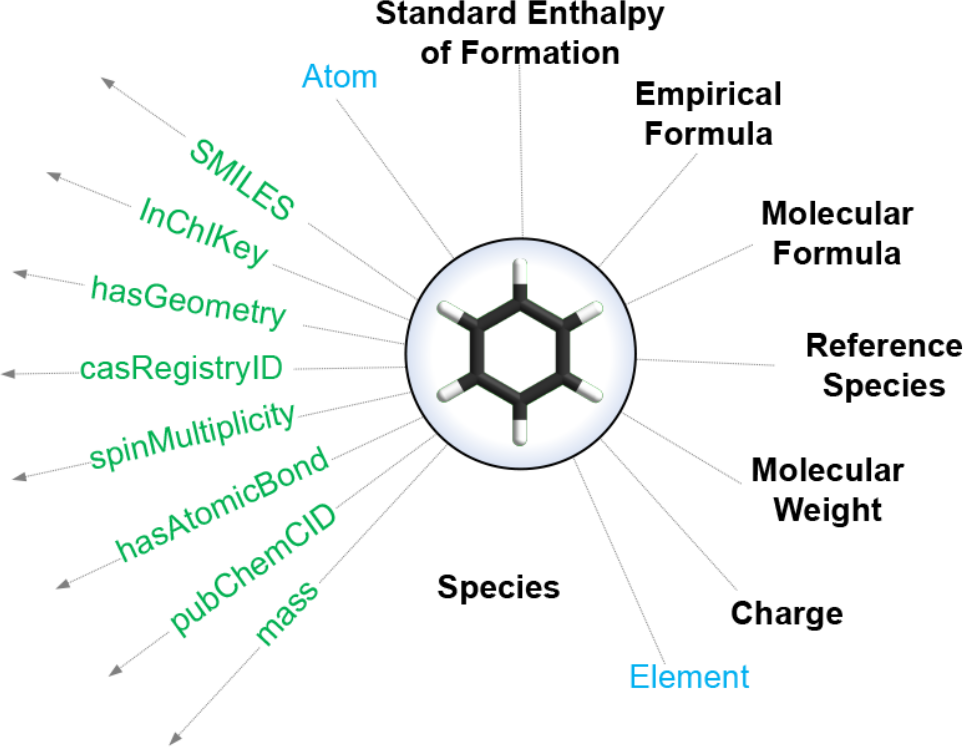
\includegraphics[height=2.10in,width=3.05in,viewport=0 0 990 750,clip]{Figures/Key_OntoSpecies-and-external_concepts.png}
\caption{\tiny\textrm{Key OntoSpecies (black) and external (blue) concepts, along with a number of properties (green) used to describe chemical species in TWA KG. cite from~\cite{ACR56-128_2023}}}%(与文献\cite{EPJB33-47_2003}图1对比)
\label{Fig:Key-OntoSpecies-and-external-concepts}
\end{figure}
}

\frame
{
	\frametitle{知识图谱的组织关系}
\begin{figure}[h!]
\centering
\vskip -8pt
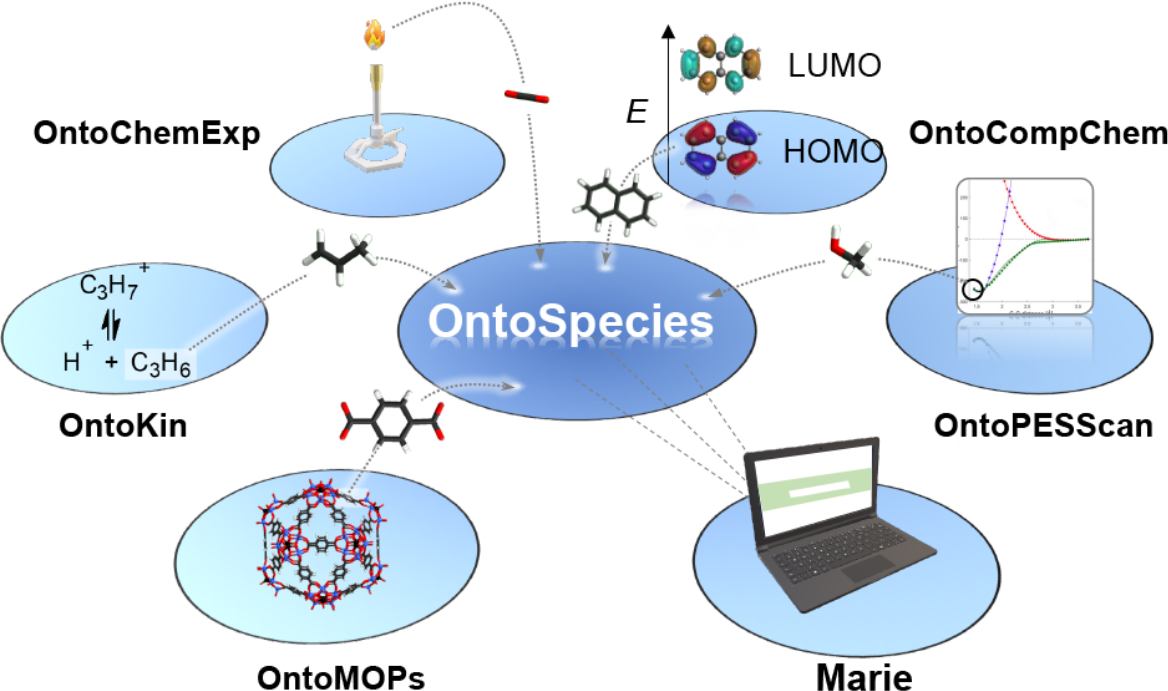
\includegraphics[height=2.45in,width=4.05in,viewport=0 0 1170 700,clip]{Figures/Connection-of-OntoSpecies-to-segments-of-KG.png}
\caption{\tiny\textrm{Connection of OntoSpecies to other segments of TWA KG. cite from~\cite{ACR56-128_2023}}}%(与文献\cite{EPJB33-47_2003}图1对比)
\label{Fig:OntoSpecies-to-segments-TWA}
\end{figure}
}

\frame
{
	\frametitle{知识的关联:~以化学物种为核心}
	通过化学物种为核心,确定相关信息的关联关系
	\begin{itemize}
		\item \textrm{OntoKin}:~表示反应机理的知识,纪录反应物、产物和反应过程的信息
		\item \textrm{OntoCompChem}:~表示计算化学的信息的知识,计算信息的描述包括
			\begin{itemize}
				\item 计算对象:~单点计算、结构优化和频率计算
				\item 计算使用的软件,{\fontsize{7.2pt}{5.2pt}\selectfont{如\textrm{Gaussian~16}}}
				\item 计算中使用的方法,包括泛函和基组{\fontsize{7.2pt}{5.2pt}\selectfont{~如\textrm{B3LYP,~6-31G(d)}}}
				\item 电荷与自旋极化
			\end{itemize}
		\item \textrm{OntoCompExp}:~表示化学实验信息的知识,包括各类化学实验条件
	\end{itemize}
\begin{thebibliography}{99}
{\tiny
\bibitem{ACR56-128_2023}\textrm{A. Kondinski, J. Bai, S. Mosbach, J. Akroyd, and M. Kraft. \textit{Acc. Chem. Res.}, \textbf{56} (2023), 128}
}
\end{thebibliography}
}

\frame
{
	\frametitle{领域知识点的描述:~\textrm{Ontology}}
	\textrm{Ontology}:~用于描述学科领域知识点的通用概念模型,模型包含学科内基本术语-术语间关系,是领域内概念的集合,\textcolor{blue}{属于群体概念}
	\begin{itemize}
		\item \textrm{Ontology}:~是哲学概念,哲学中关系的是客观存在的抽象本质
		\item 在语义学层次上,\textrm{Onlogy}是\textcolor{red}{共享概念模型的格式化规范说明}
	\begin{itemize}
		\item 共享\textrm{(Share)}:~知识必须是共同认可的
		\item 概念化\textrm{(Conceptualization)}:~对事物的描述构成一组概念
		\item 明确性\textrm{(Explicit)}:~每个术语、属性都有明确定义
		\item 格式化\textrm{(Format)}:~可以被计算机处理
	\end{itemize}
\item \textrm{Ontology}的描述语言主要有\textrm{RDF}、\textrm{RDFS}和\textrm{OWL}
	\begin{itemize}
		\item \textrm{RDF}:~用于描述\textrm{Web}上的资源\\
			用\textrm{Web}标识符来标记资源(主语),用属性(谓语)和属性值(宾语)来描述资源
		\item \textrm{RDFS}:~在\textrm{RDF}基础上扩展而成,更形象地表达知识
		\item \textrm{OWL}:~保持\textrm{RDF}、\textrm{RDFS}的兼容性,用于\textrm{ontology}的语义描述
	\end{itemize}
	\end{itemize}
}

\frame
{
	\frametitle{知识点的关联结构}
	知识图谱的关联结构:~以化学物种(元素、化合物)为核心的\textcolor{cyan}{多个知识点的\textrm{Ontology}组成}
\begin{figure}[h!]
\centering
\vskip -5pt
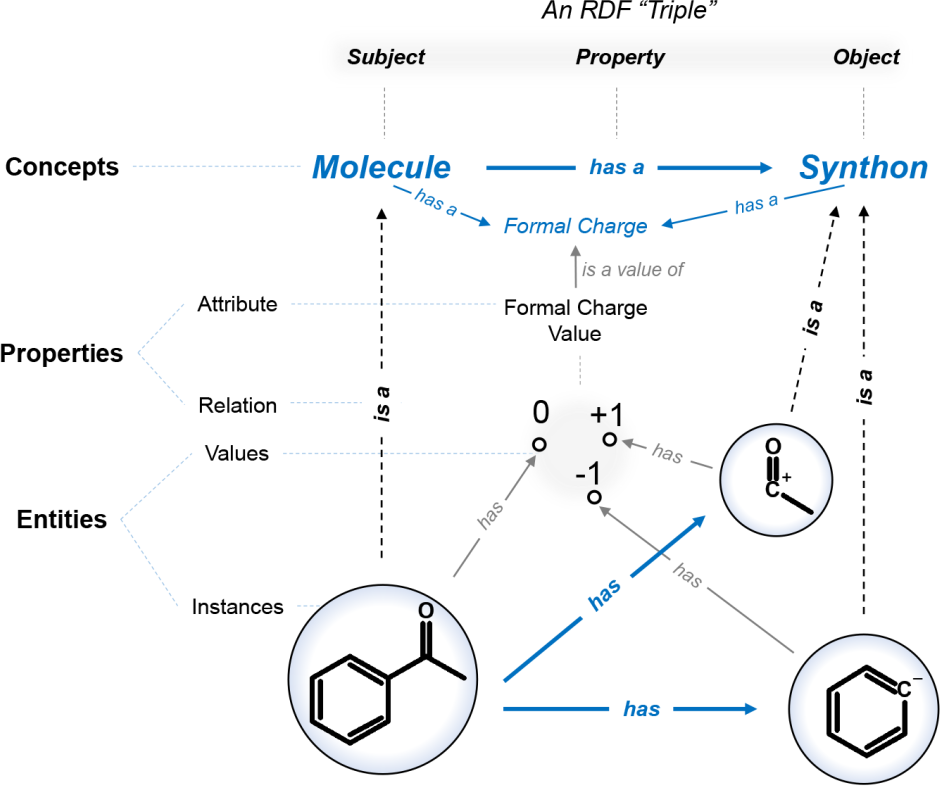
\includegraphics[height=1.70in,width=2.45in,viewport=0 0 950 790,clip]{Figures/Mapping-the-relationship-between-molecule-and-synthon.png}
\caption{\tiny\textrm{Mapping the relationship molecule (chemical) and synthon (abstract) concepts and illustrating them with instrances. cite from~\cite{ACR56-128_2023}}}%(与文献\cite{EPJB33-47_2003}图1对比)
\label{Fig:Mapping-relationship-molecule-synthon}
\end{figure}
通过数字化工具创建化学元素的基本关系,形成宏大的规划:~\\
\textcolor{red}{\textrm{TWA (The World Avatar)}}
}

\frame
{
	\frametitle{知识图谱组织示例}
\begin{figure}[h!]
\centering
\vskip -8pt
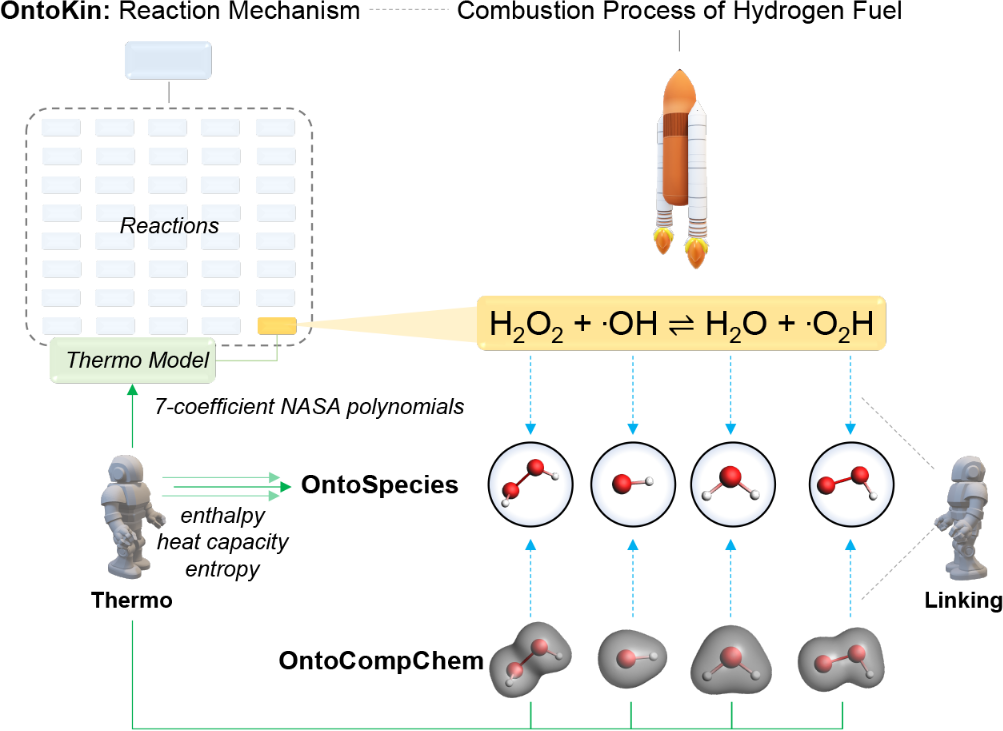
\includegraphics[height=2.50in,width=3.45in,viewport=0 0 1010 750,clip]{Figures/Automated-linking-between-OntoSepcies-Kin-CompChem.png}
\caption{\tiny\textrm{Automated linking between OntoSpecies, OntoKin and OntoCompChem. cite from~\cite{ACR56-128_2023}}}%(与文献\cite{EPJB33-47_2003}图1对比)
\label{Fig:Automated-linking-between-OntoSpecies-Kin-CompChem}
\end{figure}
}

\frame
{
	\frametitle{知识图谱组织示例}
\begin{figure}[h!]
\centering
\vskip -8pt
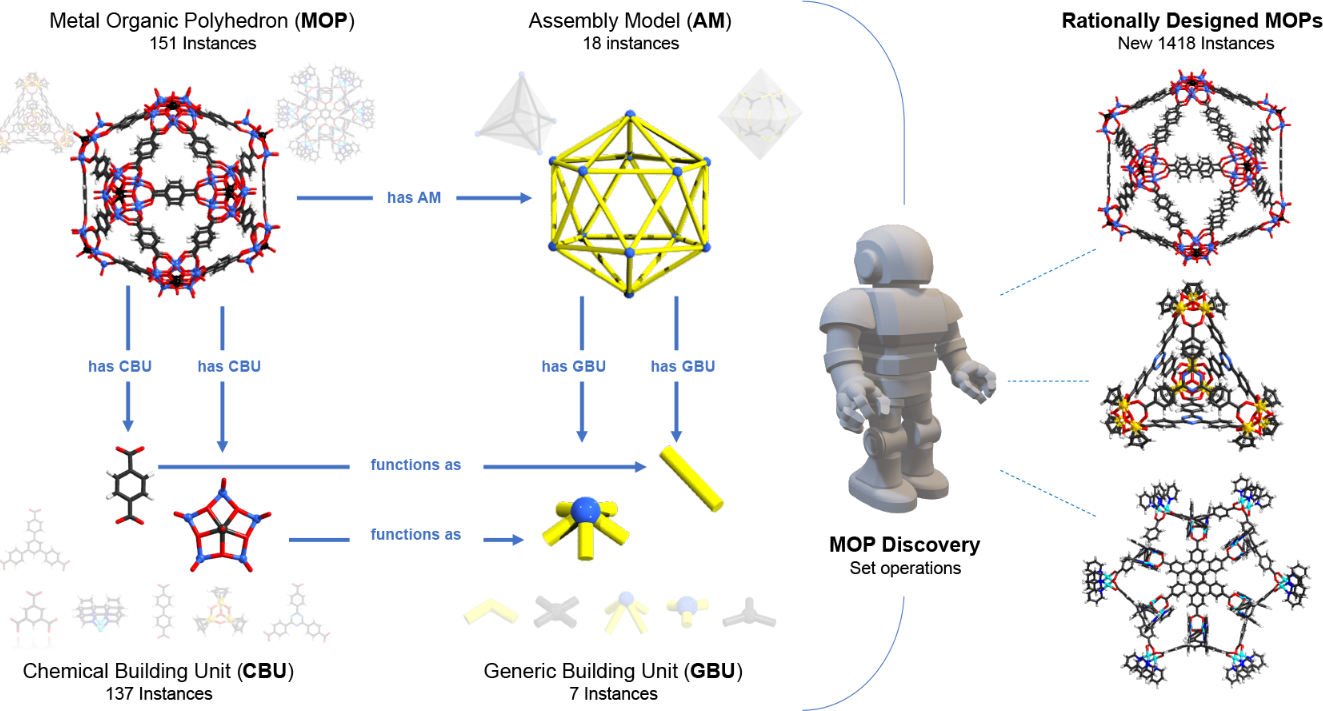
\includegraphics[height=2.20in,width=4.05in,viewport=0 0 1330 700,clip]{Figures/Key_concepts-in-OntoMOPs-and-designed-MOPs.png}
\caption{\tiny\textrm{Key concepts in OntoMOPs (left) and examples of newly rationally designed MOPs (right). cite from~\cite{ACR56-128_2023}}}%(与文献\cite{EPJB33-47_2003}图1对比)
\label{Fig:OntoMOPs-MOPs}
\end{figure}
}

\frame
{
	\frametitle{\textrm{Agent}:~化学-化工知识图谱的组织工具}
	\textrm{Agent}:~能够感知环境、进行决策和执行动作的智能处理软件
	\begin{itemize}
		\item \textrm{Agent}工作方式类似于人类代理:~能接收输入数据(如传感器信息、文本、图像等),通过分析和处理数据,理解环境和任务要求,并做出相应的决策和行动
		\item 应用场景广泛,如自动驾驶车辆、智能机器人、语音助手等
		\item \textrm{Agent}核心功能:~感知、推理和决策
			\begin{itemize}
				\item 感知:~通过传感器等方式获取环境信息的能力,例如通过摄像头获取图像或通过麦克风获取声音
				\item 推理:~基于获取的信息进行逻辑推理和分析的能力,以了解环境和任务需求
				\item 决策:~根据推理结果做出相应的决策,并执行相应的动作
			\end{itemize}
		\item 通过与环境的交互和反馈,\textrm{Agent}可以逐步改进性能和表现,实现好的任务执行能力\\
		\item \textrm{Agent}设计和训练,需要结合机器学习和人工智能技术,如强化学习、深度学习等
	\end{itemize}
}

\begin{frame}[allowframebreaks]
	\frametitle{化学-化工知识图谱的目标}
	\begin{itemize}
%	 \setlength{\itemsep}{30pt}
%{\fontsize{7.5pt}{5.5pt}\selectfont{
		\item 以化合物为核心,借助语义网\textrm{(Semantic Web)},组织、表示和存储化学-化工和领域特定类型的知识
	\item 面向碳基础材料,构建拥有学习和推理能力
		\item 具备初级的创造知识的能力,发挥人工智能的可能作用%}}
\end{itemize}
\begin{figure}[h!]
\centering
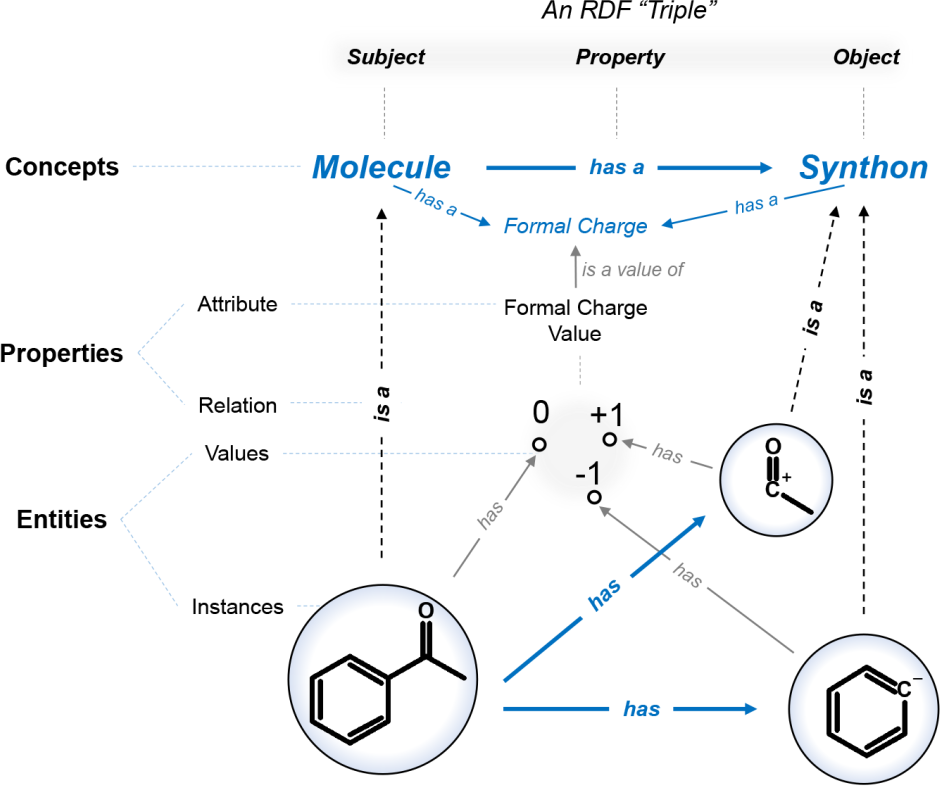
\includegraphics[height=1.50in,width=1.75in,viewport=0 0 950 790,clip]{Figures/Mapping-the-relationship-between-molecule-and-synthon.png}
\hspace{5pt}
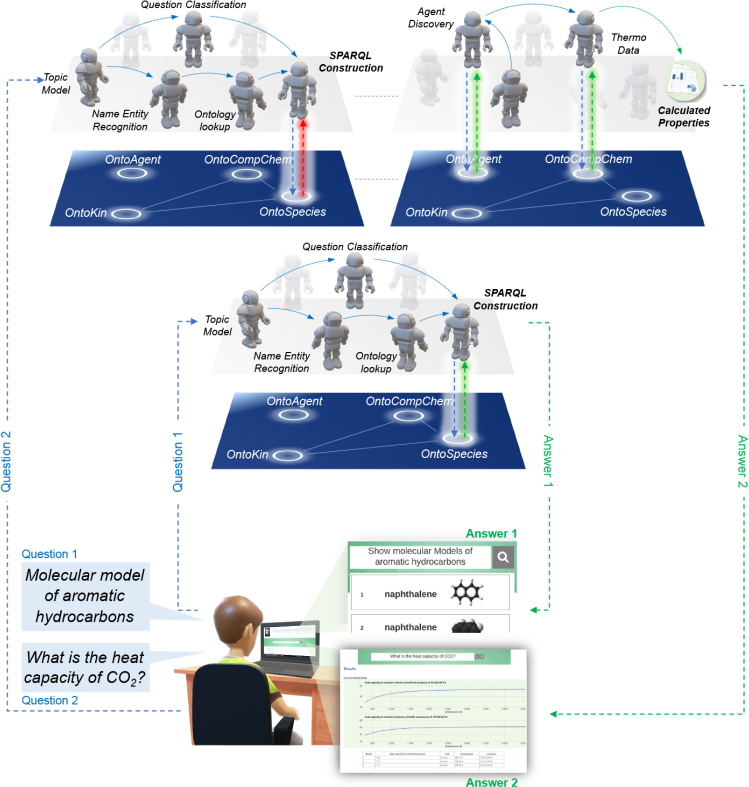
\includegraphics[height=1.50in,width=1.55in,viewport=0 0 750 790,clip]{Figures/TWA-KG-Marie.png}
%\caption{\small\textrm{Mapping the relationship molecule (chemical) and synthon (abstract) concepts and illustrating them with instrances. cite from~\cite{ACR56-128_2023}}}%(与文献\cite{EPJB33-47_2003}图1对比)
\label{Fig:Mapping-relationship-molecule-synthon-2}
\end{figure}
\textcolor{purple}{目标:}~面向人工智能的全方位转型:~智能实验室-智能科学家
\end{frame}

\section{化学-化工知识图谱}
\subsection{化学-化工知识图谱的总体目标和框架}
\frame
{
	\frametitle{化学-化工知识图谱项目的目标}
%化学-化工知识图谱项目的目标:~
	\textcolor{magenta}{通过制定化学化工数据采集方法,采用``本体-要素-概念''三位一体的技术实现业务建模,支持智慧语义认知算法和多种分析挖掘算法,完成化学-化工知识库的建设} 
\begin{itemize}
	\item \textcolor{blue}{化学-化工知识体系分类研究}:~获取其共性特征以及歧义特征\\
		{\fontsize{7.2pt}{5.2pt}\selectfont{采用标签化、智能化建立知识库的方法,主要研究知识体系、产研报告、供应链信息、原料资料、安全质量、节能环保等细分语义分类,便于在知识图谱中进行建模训练}}

\item \textcolor{blue}{行业知识数据梳理入库}\\
	{\fontsize{7.2pt}{5.2pt}\selectfont{通过百度百科、\textrm{Wiki}百科等渠道,利用数据采集系统,按研究分类自定义采集模板,将更完善的行业知识入库,有效区分结构化数据与非结构化数据的处理方案}}

\item \textcolor{blue}{构建组织表达模型}\\
	{\fontsize{7.2pt}{5.2pt}\selectfont{采用数据提取、数据整合、知识融合、知识推理、质量评估、知识存储、图谱应用等建模流程节点方案,建立一套完善、可靠的化工化学全业务知识图谱系统方案}}
\end{itemize}
\textcolor{red}{构建化学-化工行业知识图谱,为化学化工行业的研究、应用和决策提供有力支持}
}
%\subsection{化学-化工知识图谱的总体框架}
\begin{frame}
	\frametitle{化学-化工知识组织的技术实现}
	以知识图谱为例,说明(煤)化学-化工类知识采集、分类与组织
\begin{figure}[h!]
%\vspace*{-0.05in}
\centering
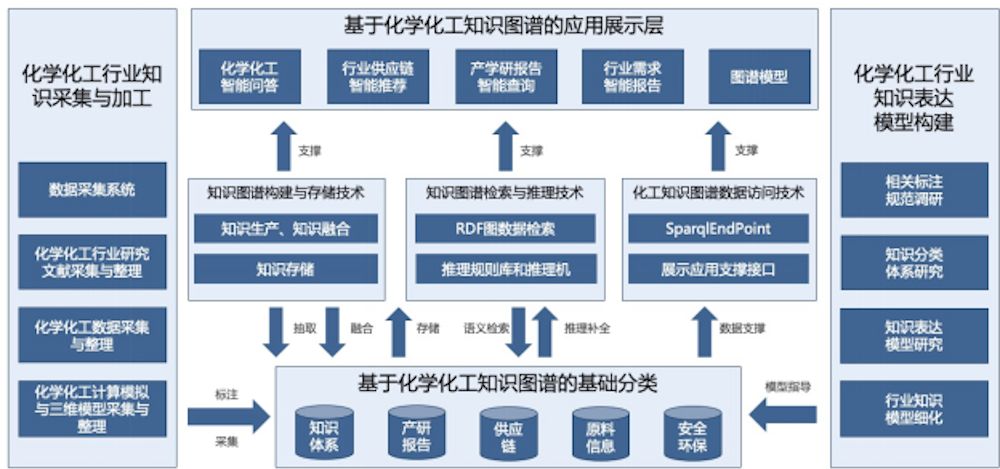
\includegraphics[height=2.08in,width=4.00in,viewport=0 0 245 113,clip]{Figures/KG_Chem-Frame.png}
\caption{\tiny 项目总体技术框架.}%(与文献\cite{EPJB33-47_2003}图1对比)
\label{KG_Chem-Frame}
\end{figure}
\end{frame}

\begin{frame}
	\frametitle{化学-化工知识的数据采集}
数据采集:~收集和整理化学-化工领域的文献、数据集、专利信息等
\begin{figure}[h!]
\centering
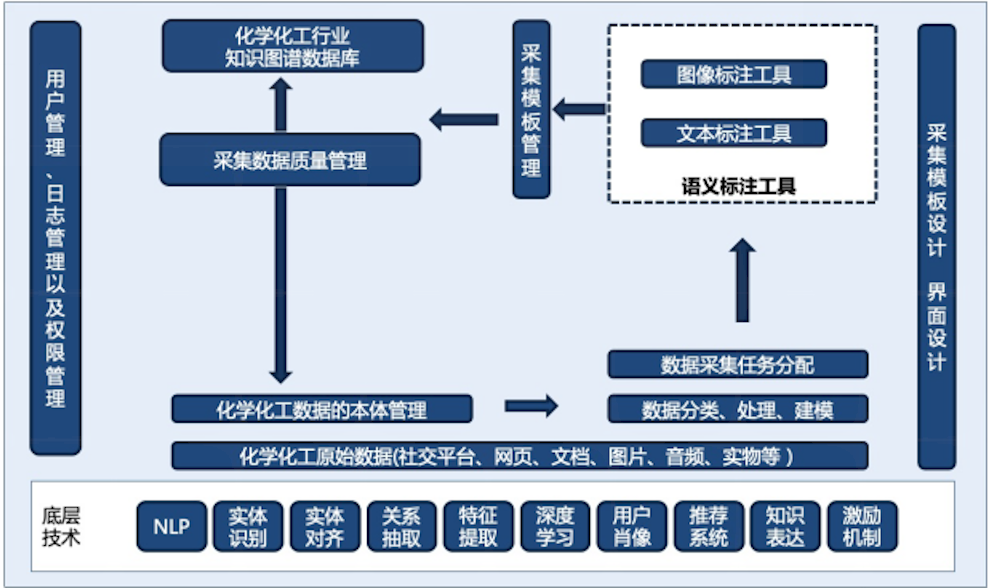
\includegraphics[height=1.80in,width=3.00in,viewport=0 0 240 150,clip]{Figures/KG_Chem-Tech_Frame.png}
\caption{\tiny 数据采集技术框架.}%(与文献\cite{EPJB33-47_2003}图1对比)
\label{KG_Chem-Tech-Frame}
\end{figure}
\vspace*{-0.1in}
\begin{itemize}
	\item {\fontsize{7.2pt}{5.2pt}\selectfont{建立规范的数据采集流程,确保数据的准确性和完整性}}
\item {\fontsize{7.2pt}{5.2pt}\selectfont{对业务进行建模,明确了化学化工领域的概念和关系,为后续知识图谱构建奠定基础}}
\end{itemize}
\end{frame}

\begin{frame}
	\frametitle{化学-化工知识库构建}
	采用本体构建技术,将领域知识转化为计算机可理解的形式:~
\begin{figure}[h!]
\centering
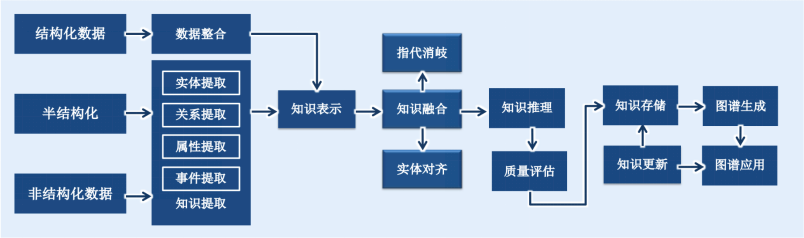
\includegraphics[height=1.30in,width=3.80in,viewport=0 0 200 57,clip]{Figures/KG_Chem-data-flow.png}
\caption{\tiny 知识表达模型和构建.}%(与文献\cite{EPJB33-47_2003}图1对比)
\label{KG_Chem-data-flow}
\end{figure}
	\begin{itemize}
		\item {\fontsize{7.2pt}{5.2pt}\selectfont{创建本体的概念、属性和关系,并进行本体的验证和优化}}
		\item {\fontsize{7.2pt}{5.2pt}\selectfont{对知识库进行了组织和分类,使用户可以方便地浏览和检索相关信息}}
	\end{itemize}
\end{frame}

\subsection{相关技术与算法}
\begin{frame}
	\frametitle{知识图谱算法提升优化}
	引入智慧语义认知算法和多种分析挖掘算法,通过对算法改进和优化,有效提升知识图谱的智能化和实用性
	\vskip 20pt
	\begin{itemize}
	 \setlength{\itemsep}{15pt}
		\item \textcolor{blue}{智慧语义认知算法}\\
能够理解用户的查询意图,可提供更准确和个性化的搜索结果
\item \textcolor{blue}{分析挖掘算法}\\
	从大量的数据中发现隐藏的关联和规律,为化学-化工行业的研究和决策提供有价值的信息
	\end{itemize}
\end{frame}

\begin{frame}[allowframebreaks]
	\frametitle{化学-化工行业数据采集与加工算法}
	自然语言表述(非结构化数据)$\Longrightarrow$结构化数据
	\vskip 2pt
数据来源:
	\begin{itemize}
		\item 基础数据来源:~教科书录入\& 爬虫技术\textrm{(Web Crawle)}获取
		\item \textcolor{red}{由专业人员提供}:~行业研究文献采集与梳理
		\item 化学-化工计算模拟与三维模型采集与整理(\textcolor{red}{规划中}) 
	\end{itemize}

	文本分词与句读标注:\vskip 2pt
			%清华大学自然语言处理与社会人文计算实验室研制推出的
	\textcolor{blue}{\textrm{thulac}}:~{\fontsize{7.2pt}{5.2pt}\selectfont{一套中文词法分析工具包,具有中文分词和词性标注功能}}
	\begin{itemize}
		\item 能力强\\
			{\fontsize{6.2pt}{5.2pt}\selectfont{利用目前世界上规模最大的人工分词和词性标注中文语料库(约含5800万字)训练而成,模型标注能力强大}}
		\item 准确率高\\
			{\fontsize{7.2pt}{5.2pt}\selectfont{该工具包在标准数据集Chinese Treebank(CTB5)上分词的\textrm{F1}值可达97.3\%,词性标注的\textrm{F1}值可达到92.9\%,与该数据集上最好方法效果相当}}
	\item 速度较快\\
		{\fontsize{7.2pt}{5.2pt}\selectfont{同时进行分词和词性标注速度为300\textrm{KB/s},每秒可处理约15万字。只进行分词速度可达到\textrm{1.3MB/s}}}
	\end{itemize}

	实体关系分类:\vskip 2pt
	\textcolor{blue}{\textrm{fastText}}:~快速文本分类
	\begin{itemize}
		\item 结合了自然语言处理和机器学习中最成功的理念\\
			{\fontsize{6.2pt}{5.2pt}\selectfont{包括使用词袋以及\textrm{n-gram}袋表征语句,使用子字\textrm{(subword)}信息,并通过隐藏表征在类别间共享信息}}
		\item 采用\textrm{softmax}层级(利用了类别不均衡分布的优势)来加速
		\item 在保持高精度的情况下加快了训练速度和测试速度
		\item 不需要预训练好的词向量,会自己训练词向量
	\end{itemize}

	\textcolor{blue}{\textit{k}-\textrm{NN}}算法:~定义页面的相似度
\begin{itemize}
	\item 计算\textrm{title}之间的词向量的余弦相似度(利用\textrm{fastText}计算的词向量能够避免\textrm{out of vocabulary})
	\item 计算两组\textrm{openType}之间的词向量的余弦相似度的平均值
	\item 计算具有相同的\textrm{baseInfoKey}的\textrm{IDF}值之和(因为`中文名'这种属性贡献应该比较小)
	\item 统计具有相同\textrm{baseInfoKey}下\textrm{baseInfoValue}相同的个数
\end{itemize}
预测一个页面时,由于\textrm{kNN}要将该页面和训练集中所有页面进行比较,因此每次预测的复杂度是$O(n)$,$n$为训练集规模。在这个过程中,可以统计各个分相似度的\textrm{IDF}值、均值、方差、标准差,然后对4个相似度进行标准化:
		\begin{displaymath}
			(x-\bar{x})/\mathrm{D}(x)
		\end{displaymath}
		这里$\bar{x}$是均值,$\mathrm{D}(x)$是方差\\
	上述四个部分的相似度的加权和为最终的两个页面的相似度,权值由向量\textrm{weight}控制,通过10折叠交叉验证$+$网格搜索得到
%\begin{figure}[h!]
%%\vspace*{-0.05in}
%\centering
%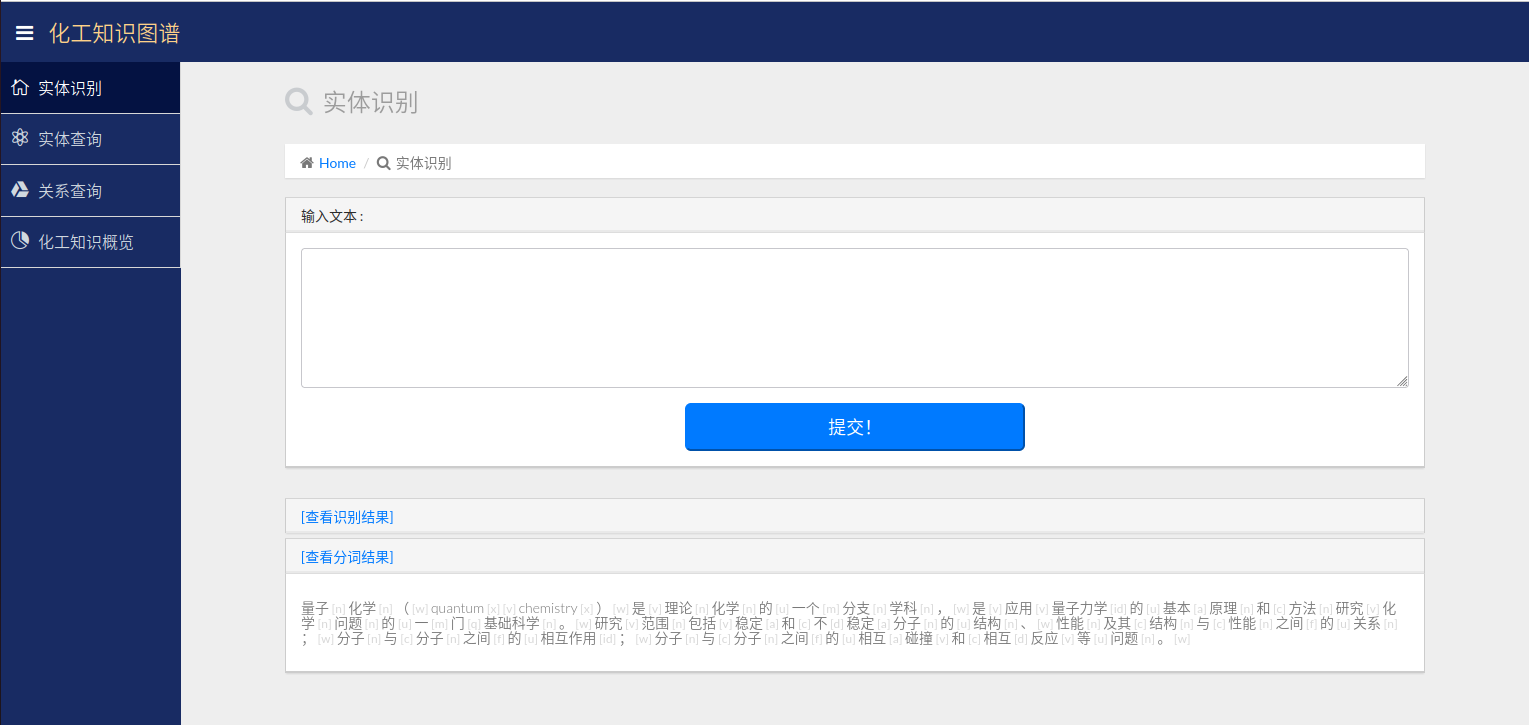
\includegraphics[height=1.58in,width=3.00in,viewport=0 0 1529 725,clip]{Figures/KG_Chem-word_segmentation.png}
%\caption{\tiny 自然语言的数据提取.}%(与文献\cite{EPJB33-47_2003}图1对比)
%\label{KG_Chem-word_segmentation}
%\end{figure}
\end{frame}

\begin{frame}
	\frametitle{化学-化工领域数据采集}
%	针对化学化工相关信息多源异构难以获取的问题,
	基于网络爬虫技术实现多源数据信息的分布式爬虫,获取相关信息,训练并扩大,形成相对结构化的化学-化工信息语料库 
\begin{figure}[h!]
\centering
\vskip -8pt
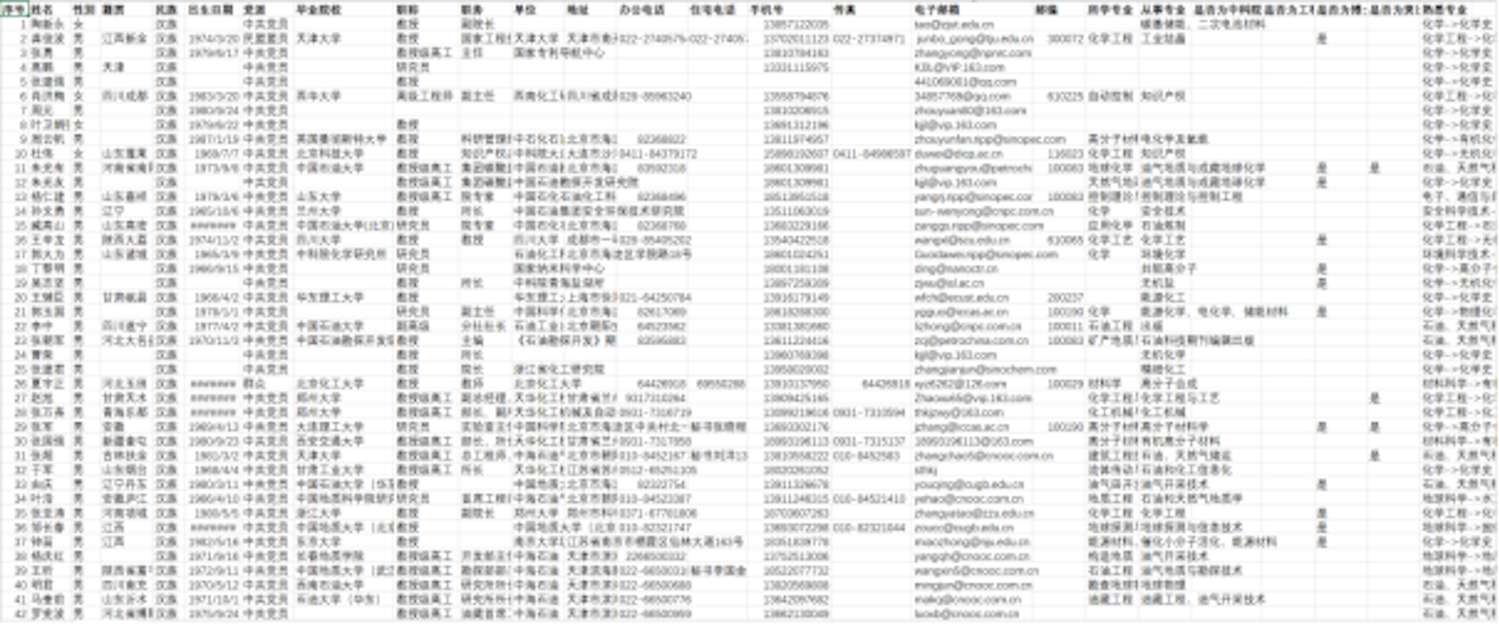
\includegraphics[height=2.10in,width=4.00in,viewport=0 0 210 95,clip]{Figures/KG_Chem-Info.png}
\caption{\tiny 有组织的数据是一切\textrm{AI}知识的基础}%(与文献\cite{EPJB33-47_2003}图1对比)
\label{Fig:KG_Chem-Info}
\end{figure}
\end{frame}

\begin{frame}
	\frametitle{化学-化工领域细粒度领域分类}
化学-化工专家文档以层级结构为特征,通过神经网络可抽取文档上下文层级语义关系:~
根据专家简介词、句、段落文档层级结构特征,分层捕获文档之间的语义关系,实现化学化工领域细粒度分类
\begin{figure}[h!]
\centering
%\vskip -8pt
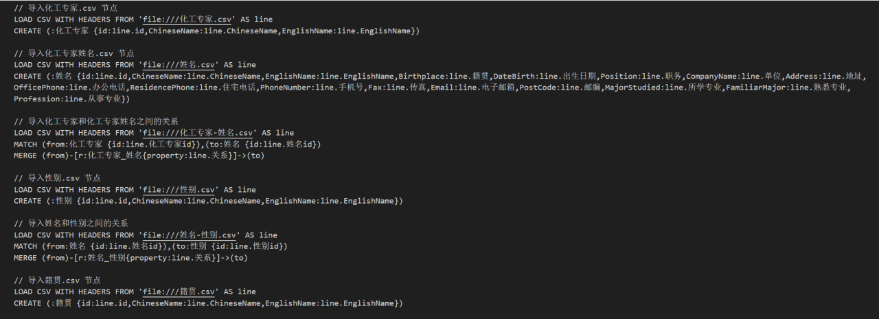
\includegraphics[height=1.60in,width=4.00in,viewport=0 0 210 80,clip]{Figures/KG_Chem-extract.png}
\caption{\tiny 专家简介文档层级结构特征分层,用于捕获文档之间语义关系}%(与文献\cite{EPJB33-47_2003}图1对比)
\label{Fig:KG_Chem-Extract}
\end{figure}
\textcolor{red}{神经网络分类器在获取文档语义关系中取得了很好的效果}
\end{frame}

\subsection{化学化工知识图谱的建设}
\begin{frame}
	\frametitle{结构化数据关系提取}
	对数据集处理,得到关系抽取需要用到的\textrm{json}文件
\begin{itemize}
	\item 用公开数据集测试%如果当前文件夹下没有`filter_train_data_all_deduplication.txt`, 那么进入wikidataSpider目录,根据TrainDataBaseOnWiki/readme.md中所述方法,获得`filter_train_data_all_deduplication.txt` (生成数据时间比较长,建议用公开数据集测试。使用公开数据集,直接从进入Algorithm,忽略之后所有的操作)
	\item 数据清洗\textrm{filter dataset}
	%* 运行`python dosomething.py filter_dataset` 得到`filtered_data.txt` 
	\item 获得关系与\textrm{id}的关系:~\textrm{rel2id}数据库
	%* 运行`python preprocessing.py rel2id` 得到rel2id.json
	\item 获得数据集:~\textrm{dataset}数据库
%* 运行`python preprocessing.py dataset.json`得到dataset.json
	\item 获得数据
%* 运行`python preprocessing.py word2vecjson` 得到word2vec.json
	\item 获得实体与\textrm{id}的关系:~\textrm{entity2id}数据库
%* 运行`python preprocessing.py entity2id`得到entity2id.json
	\item 获得训练数据集和测试数据集
%* 运行`python preprocessing.py dataset_split`得到train_dataset.json和test_dataset.json
\end{itemize}
\end{frame}

\begin{frame}
	\frametitle{实体识别}
	\begin{itemize}
	 \setlength{\itemsep}{10pt}
		\item 命名实体类型多样,数量众多,不断有新的命名实体涌现,如新的人名、地名等
		\item 命名实体构成结构比较复杂,某些类型的命名实体词的长度没有一定的限制
\item 在不同领域、场景,命名实体的外延有差异,可能产生歧义
	\end{itemize}
	\begin{tikzpicture}[
    box/.style={rectangle,draw,fill=darkgray!20,node distance=1cm,text width=15em,text centered,rounded corners,minimum height=2em,thick},
    arrow/.style={draw,-latex',thick},]
    \node [box, text width=5em] (apple-orig) {\huge{苹果}};
    \node [box, text=red, above=1.0 of apple-orig, text width=12em] at (6.5, 0.0) (apple-fruit) {\huge{\textrm{苹果(水果)}}};
    \node [box, text=blue, below=2.0 of apple-fruit, text width=12em] (apple-coop) {\huge{\textrm{苹果公司}}};
%\node at (-5,0) (Figure){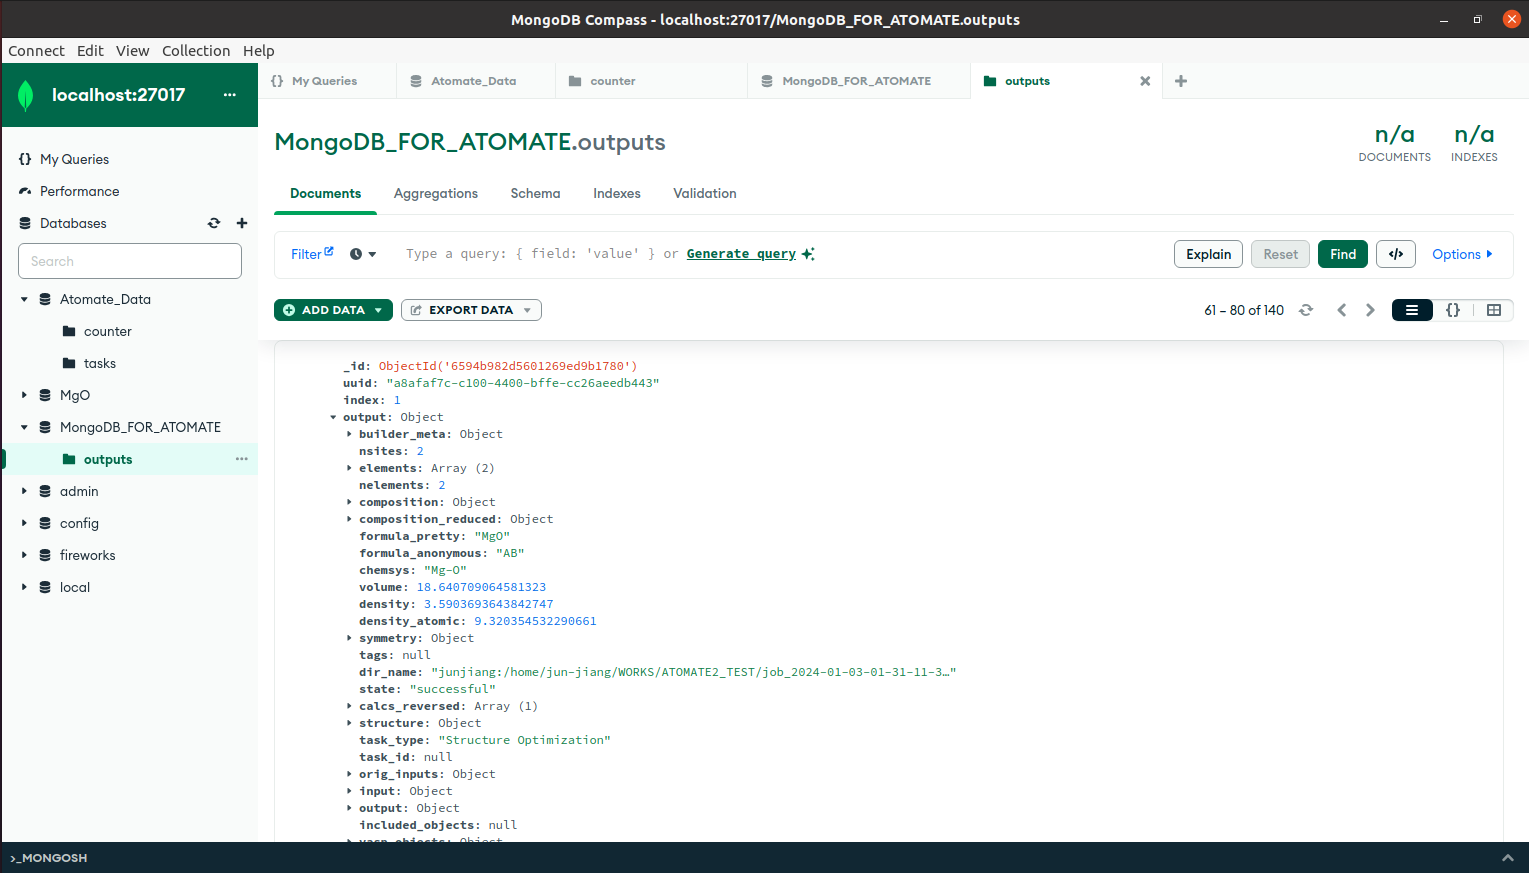
\includegraphics[height=2.35in,width=4.05in,viewport=0 0 1529 873,clip]{Figures/Database_Materials.png}};
  \path [arrow] (apple-orig.east) -- (apple-fruit.west);
  \path [arrow] (apple-orig.east) -- (apple-coop.west);
%\caption{\tiny \textrm{中文语句中实体识别的示例.}}%(与文献\cite{EPJB33-47_2003}图1对比)
\end{tikzpicture}
\end{frame}

\begin{frame}
	\frametitle{示例:~实体识别}
	\begin{tikzpicture}[
    box/.style={rectangle,draw,fill=darkgray!20,node distance=1cm,text width=15em,text centered,rounded corners,minimum height=2em,thick},
    arrow/.style={draw,-latex',thick},]
    \node [box, text width=28em] (Sentence) {\huge{李群生、王建翔在北京参加中国化学会会议}};
    \node [box, text=red, above=2.5 of Sentence, text width=12em] at (-1.0, 0.0) (Person) {\huge{\textrm{Per}}};
    \node [box, text=blue, right=1.0 of Person, text width=5em] (Location) {\huge{\textrm{Loc}}};
    \node [box, text=magenta, below=1.5 of Sentence, text width=6em] (Organization) {\huge{\textrm{Org}}};
%\node at (-5,0) (Figure){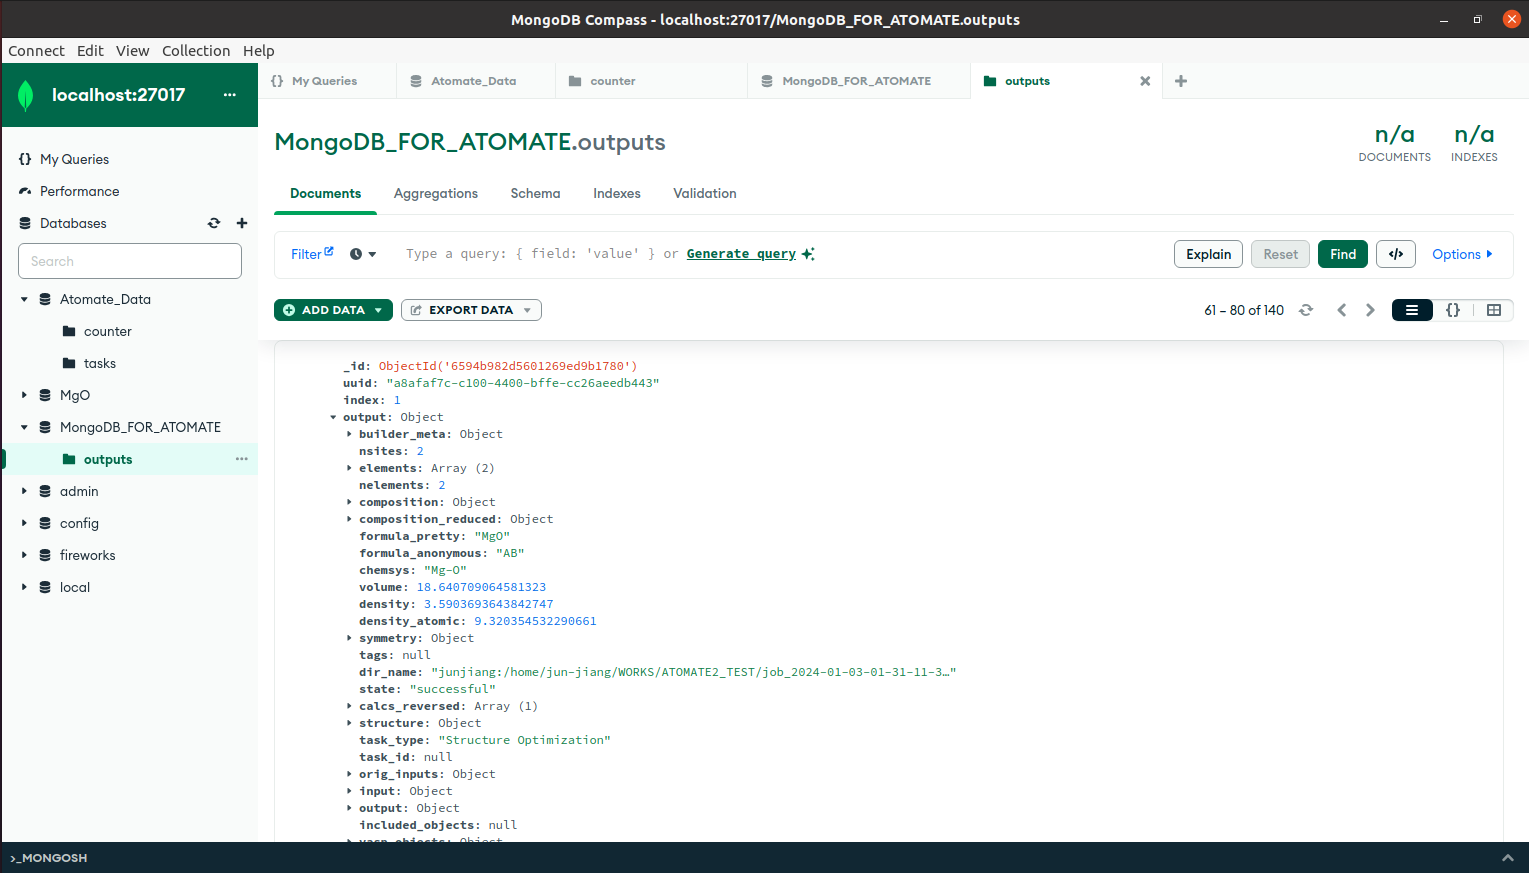
\includegraphics[height=2.35in,width=4.05in,viewport=0 0 1529 873,clip]{Figures/Database_Materials.png}};
  \path
  (Sentence.north west) ++(3.8em,-1.1em) coordinate (Li-left fit)
  (Sentence.north west) ++(8.8em,-1.6em) coordinate (Li-right fit)
  (Sentence.north west) ++(12.9em,-1.1em) coordinate (Wang-left fit)
  (Sentence.north west) ++(18.0em,-1.6em) coordinate (Wang-right fit)
  (Sentence.north west) ++(22.1em,-1.1em) coordinate (Peking-left fit)
  (Sentence.north west) ++(25.1em,-1.6em) coordinate (Peking-right fit)
  (Sentence.north west) ++(9.4em,-3.1em) coordinate (ACC-left fit)
  (Sentence.north west) ++(19.6em,-3.7em) coordinate (ACC-right fit);

\node[rectangle,draw=red, dashdotted, inner sep=0.75em, fit=(Li-left fit) (Li-right fit)] (enclosure1) {};
\node[rectangle,draw=red, dashdotted, inner sep=0.75em, fit=(Wang-left fit) (Wang-right fit)] (enclosure2) {};
\node[rectangle,draw=blue, dashdotted, inner sep=0.75em, fit=(Peking-left fit) (Peking-right fit)] (enclosure3) {};
\node[rectangle,draw=magenta, dashdotted, inner sep=0.75em, fit=(ACC-left fit) (ACC-right fit)] (enclosure4) {};
  \path [arrow, fill=red] (enclosure1) -- (Person);
  \path [arrow,fill=red] (enclosure2) -- (Person);
  \path [arrow,fill=blue] (enclosure3) -- (Location);
  \path [arrow,fill=magenta] (enclosure4) -- (Organization);
%\caption{\tiny \textrm{中文语句中实体识别的示例.}}%(与文献\cite{EPJB33-47_2003}图1对比)
\end{tikzpicture}
\end{frame}

\begin{frame}
	\frametitle{自然语言处理框架}
\begin{figure}[h!]
\centering
%\vskip -8pt
\includegraphics[height=2.00in,width=4.00in,viewport=0 0 200 90,clip]{Figures/KG_Chem-NL_frame.png}
\caption{\tiny 自然语言处理的技术流程}%(与文献\cite{EPJB33-47_2003}图1对比)
\label{Fig:KG_Chem-NL_frame}
\end{figure}
\end{frame}

\begin{frame}
	\frametitle{\textrm{kNN}}
\begin{figure}[h!]
\centering
\vskip -8pt
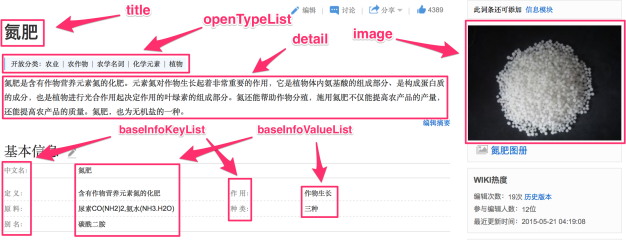
\includegraphics[height=1.10in,width=2.70in,viewport=0 0 150 60,clip]{Figures/KG_Chem-Nitro_fertilizer.png}
\caption{\tiny 自然语言处理的技术应用示范}%(与文献\cite{EPJB33-47_2003}图1对比)
\label{Fig:KG_Chem-Nitro_fertilizer}
\end{figure}
\begin{itemize}
	\item {\fontsize{7.2pt}{6.2pt}\selectfont{\textrm{title}间词向量的余弦相似度}}
	\item {\fontsize{7.2pt}{6.2pt}\selectfont{\textrm{openTypeList}之间词向量的余弦相似度的平均值}}
	\item {\fontsize{7.2pt}{6.2pt}\selectfont{\textrm{detail}之间比较文档向量的预选相似度}}
	\item {\fontsize{7.2pt}{6.2pt}\selectfont{\textrm{baseInfoKeyList}之间的\textrm{IDF}值之和}}
	\item {\fontsize{7.2pt}{6.2pt}\selectfont{相同\textrm{baseInfoKey}下\textrm{baseInfoValue}相同的个数}}
	\item {\fontsize{7.2pt}{6.2pt}\selectfont{各项指标进行标准化,使其都服从均值为$0$,方差为$1$的分布}}
	\item {\fontsize{7.2pt}{6.2pt}\selectfont{各项指标进行加权求和,权值通过交叉验证$+$网格搜索求得}}
\end{itemize}
\end{frame}

\begin{frame}
	\frametitle{关系抽取}
	关系抽取是从语句中获取实体之间关系的一种技术
%实体对应知识图谱中的结点,关系则对应知识图谱中的边
%文本语句的结构复杂,人工制定规则工作量巨大
%不同语言、不同领域之间存在差异,人工制定规则难以迁移
\begin{figure}[h!]
\centering
\vskip -8pt
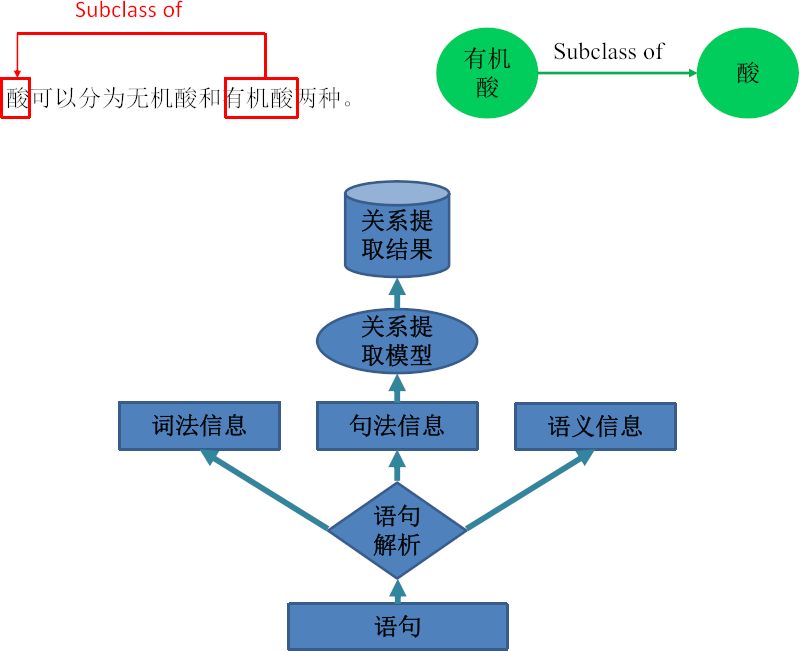
\includegraphics[height=2.00in,width=2.40in,viewport=0 0 200 170,clip]{Figures/KG_Chem-Relation_extract.png}
\caption{\tiny 关系抽取技术框架}%(与文献\cite{EPJB33-47_2003}图1对比)
\label{Fig:KG_Chem-Relation_extract}
\end{figure}
有监督学习方法进行关系提取,人工标注训练样本成本巨大\\\textcolor{red}{如何获得足够多的高质量训练样本是一大难题}
\end{frame}

\begin{frame}
	\frametitle{化学-化工知识关系抽取模型}
	应用\textrm{PCNNs}模型进行关系预测
\begin{figure}[h!]
\centering
%\vskip -8pt
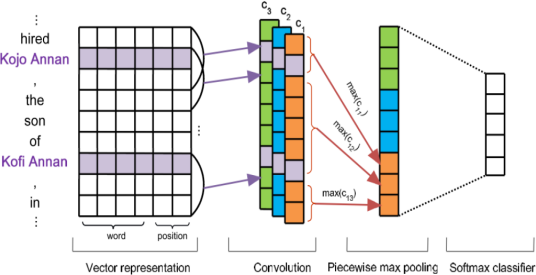
\includegraphics[height=2.10in,width=4.00in,viewport=0 0 130 70,clip]{Figures/KG_Chem-PCNNs.png}
\caption{\tiny 化学-化工知识关系抽取模型}%(与文献\cite{EPJB33-47_2003}图1对比)
\label{Fig:KG_Chem-PCNNs}
\end{figure}
\end{frame}

\begin{frame}
	\frametitle{总体架构}
\begin{minipage}[b]{0.48\textwidth}
\begin{figure}[h!]
\centering
%\vskip -8pt
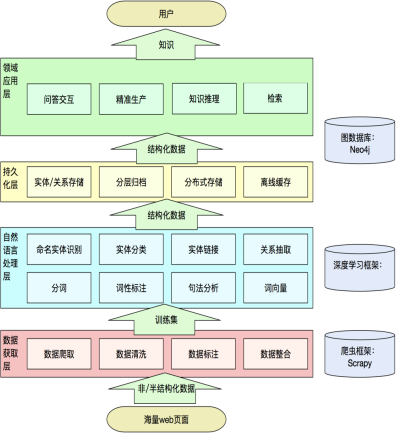
\includegraphics[height=2.00in,width=1.50in,viewport=0 0 95 110,clip]{Figures/KG_Chem-Frame_Relation.png}
\caption{\tiny 化学-化工知识图谱总体架构}%(与文献\cite{EPJB33-47_2003}图1对比)
\label{Fig:KG_Chem-Frame_Relation}
\end{figure}
\end{minipage}
\begin{minipage}[c]{0.50\textwidth}
\vspace*{-2.15in}
	当前语料数据库规模
\begin{itemize}%[+-| alert@+>]
 {\fontsize{7.5pt}{6.0pt}\selectfont
%	 \setlength{\itemsep}{10pt}
 \item 语料库大小:~\textrm{10GB$+$}
 \item 实体数量:~\textrm{3W$+$}
 \item 关系数量:~\textrm{4W$+$}}
\end{itemize}
关键问题
\begin{itemize}%[+-| alert@+>]
 {\fontsize{7.5pt}{6.0pt}\selectfont
%	 \setlength{\itemsep}{10pt}
 \item 大规模语料库获取
 \item 大规模的算法训练
 \item 大量的实体和关系存储}
\end{itemize}
解决方案:
\begin{itemize}%[+-| alert@+>]
 {\fontsize{7.5pt}{6.0pt}\selectfont
%	 \setlength{\itemsep}{10pt}
\item 采用分布式爬虫框架
\item 采用支持\textrm{GPU}加速的框架:~\textrm{Pytorch}
\item 采用分布式图数据库:~\textrm{Neo4j}}
\end{itemize}
\end{minipage}
\end{frame}

\begin{frame}
	\frametitle{\textrm{Scrapy}:~分布式爬虫框架}
\begin{figure}[h!]
\centering
\vskip -8pt
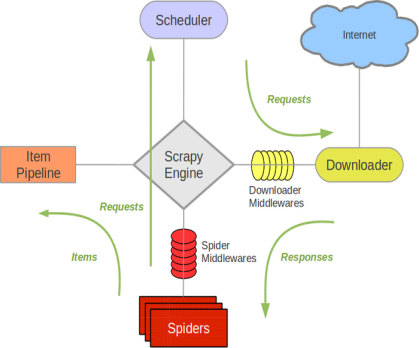
\includegraphics[height=1.20in,width=2.30in,viewport=0 0 115 90,clip]{Figures/KG_Chem-Scrapy.png}
\caption{\tiny \textrm{scrapy}爬虫框架}%(与文献\cite{EPJB33-47_2003}图1对比)
\label{Fig:KG_Chem-scrapy}
\end{figure}
\textrm{Scrapy}爬虫的执行
\begin{itemize}
 {\fontsize{7.5pt}{6.0pt}\selectfont
	\item 引擎从调度器中取出一个链接\textrm{(URL)}用于接下来的抓取
	\item 引擎把\textrm{URL}封装成一个请求\textrm{(Request)}传给下载器
	\item 下载器把资源下载下来,并封装成应答包\textrm{(Response)}
	\item 爬虫解析\textrm{Response}
	\item 解析出实体\textrm{(Item)},则交给实体管道进行进一步的处理
	\item 解析出的是链接\textrm{(URL)},则把\textrm{URL}交给调度器等待抓取}
\end{itemize}
\end{frame}

\begin{frame}
	\frametitle{\textrm{Pytorch}:~深度学习框架}
\begin{figure}[h!]
\centering
\vskip -8pt
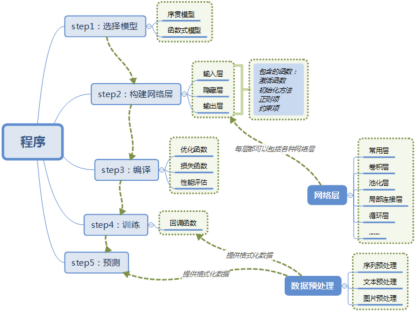
\includegraphics[height=2.00in,width=2.40in,viewport=0 0 110 80,clip]{Figures/KG_Chem-Pytorch.png}
\caption{\tiny \textrm{scrapy}爬虫框架}%(与文献\cite{EPJB33-47_2003}图1对比)
\label{Fig:KG_Chem-Pytorch}
\end{figure}
利用\textrm{Pytorch}框架和高性能\textrm{GPU}资源,提升神经网络的训练速度
\end{frame}

\begin{frame}
	\frametitle{\textrm{Neo4j}:~大规模图形存储}
	\begin{itemize}
		\item 对于大规模的结点和边的存储和运算,传统关系型数据库\textrm{(例如MySQL)}效率低下%;而Neo4j则很好的支持高效的图运算
		\item 传统的图运算都是在内存中进行的,当内存较小时,往往无法加载整个知识图谱
		\item 采用\textrm{Neo4j},服务器能在磁盘中进行图运算 
	\end{itemize}
	\textrm{Neo4j}使用的查询语言为\textrm{Cypher},\textrm{Cypher}是描述性的图形查询语言,语法简单,功能强大
	\begin{itemize}
		\item 在结点和关系数量庞大的图形中,有更快的数据库操作速度
		\item 支持分布式存取,能够利用集群来扩展内存和磁盘容量
		\item 支持分布式高可用性,可支持大规模的数据增长
		\item 数据安全可靠,支持数据的实时备份
		\item \textrm{Cypher}语句使图数据的操作与展示更直观
	\end{itemize}
\end{frame}

\begin{frame}
	\frametitle{示例:~\textrm{Neo4j}}
\begin{figure}[h!]
\centering
\vskip -8pt
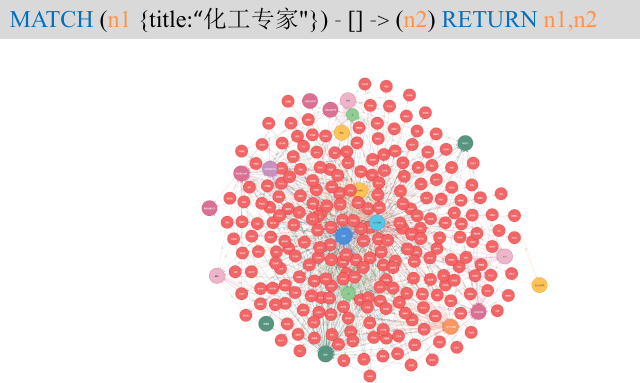
\includegraphics[height=2.20in,width=3.40in,viewport=0 0 150 100,clip]{Figures/KG_Chem-Neo4j.png}
\caption{\tiny 化学-化工图谱中的\textrm{neo4j}示例}%(与文献\cite{EPJB33-47_2003}图1对比)
\label{Fig:KG_Chem-Neo4j}
\end{figure}
%利用\textrm{Pytorch}框架和高性能\textrm{GPU}资源,提升神经网络的训练速度
\end{frame}

\begin{frame}
	\frametitle{知识图谱\textrm{RDF}图数据检索}
\begin{figure}[h!]
\centering
%\vskip -8pt
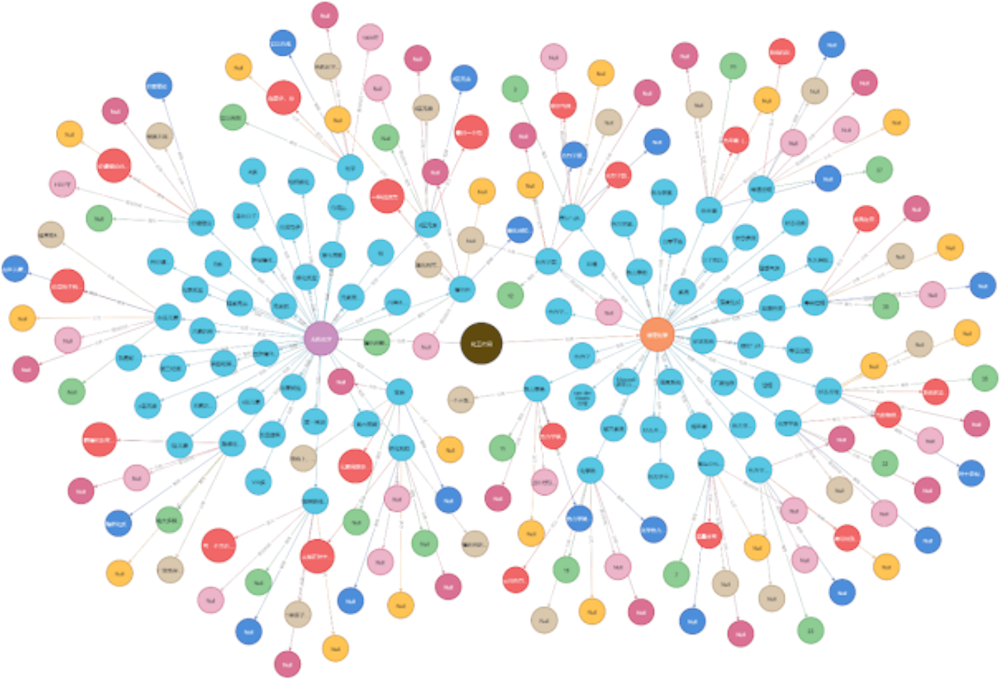
\includegraphics[height=2.60in,width=4.00in,viewport=0 0 240 180,clip]{Figures/KG_Chem-Inorganic.png}
\caption{\tiny 知识图谱的数据\textrm{RDF}图:~无机化合物}%(与文献\cite{EPJB33-47_2003}图1对比)
\label{Fig:KG_Chem-Inorganic}
\end{figure}
\end{frame}

\begin{frame}
	\frametitle{知识图谱\textrm{RDF}图数据:~示例}
\begin{figure}[h!]
\centering
%\vskip -8pt
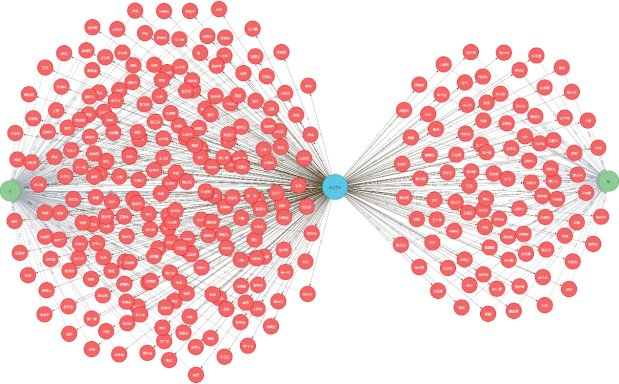
\includegraphics[height=2.40in,width=4.00in,viewport=0 0 150 100,clip]{Figures/KG_Chem-Chemist.png}
\caption{\tiny 知识图谱的数据\textrm{RDF}图:~化工专家-姓名-性别}%(与文献\cite{EPJB33-47_2003}图1对比)
\label{Fig:KG_Chem-Chemist}
\end{figure}
\end{frame}

\begin{frame}
	\frametitle{知识图谱\textrm{RDF}图数据:~示例}
\begin{figure}[h!]
\centering
%\vskip -8pt
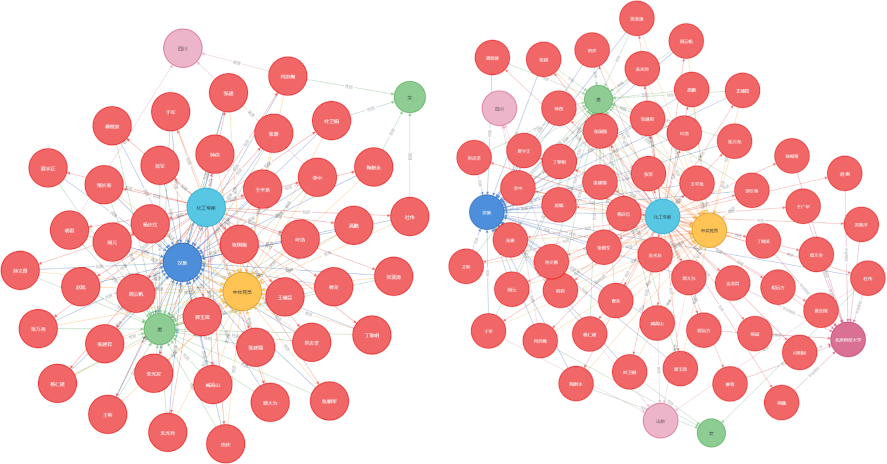
\includegraphics[height=2.10in,width=4.00in,viewport=0 0 220 115,clip]{Figures/KG_Chem-Chemist_2.png}
\caption{\tiny 知识图谱的数据\textrm{RDF}图:~化工专家-姓名-身份-学历}%(与文献\cite{EPJB33-47_2003}图1对比)
\label{Fig:KG_Chem-Chemist2}
\end{figure}
\end{frame}

\begin{frame}
	\frametitle{化学-化工知识图谱:~示例}
\begin{figure}[h!]
\centering
%\vskip -8pt
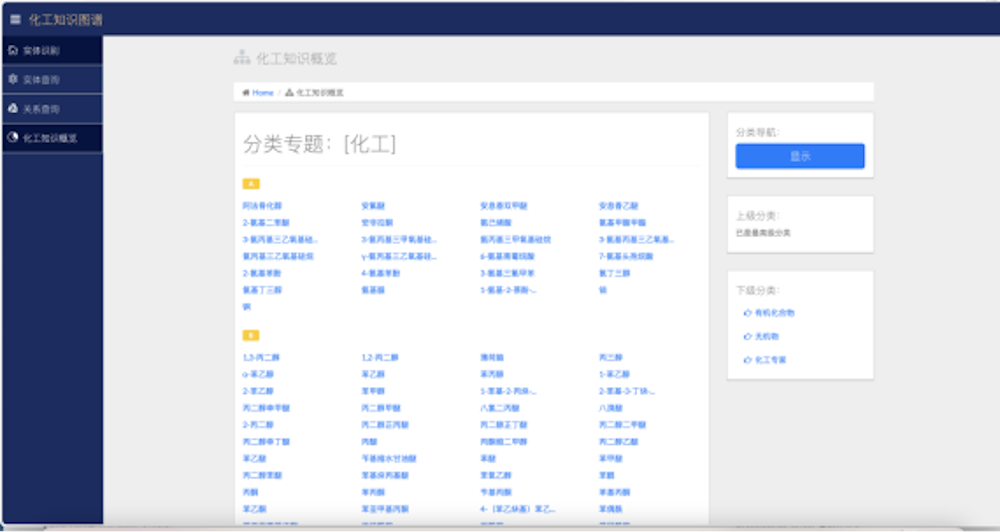
\includegraphics[height=2.10in,width=4.00in,viewport=0 0 240 130,clip]{Figures/KG_Chem-html.png}
\caption{\tiny 化学-化工知识图谱网页}%(与文献\cite{EPJB33-47_2003}图1对比)
\label{Fig:KG_Chem-Enflurane}
\end{figure}
\end{frame}

\begin{frame}
	\frametitle{化学-化工知识图谱:~界面}
\begin{figure}[h!]
\centering
\vskip -8pt
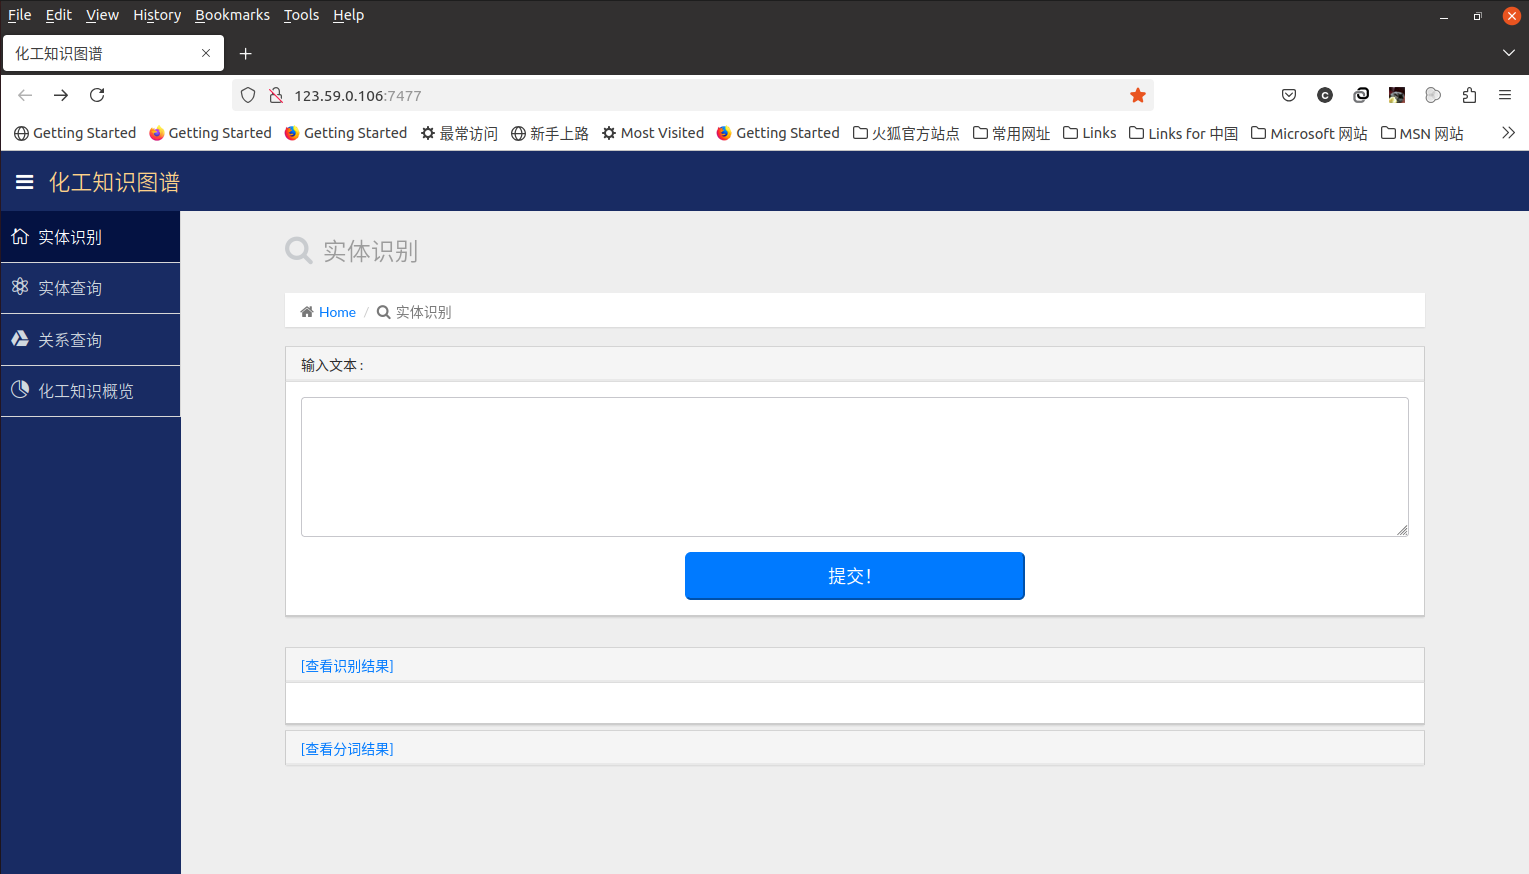
\includegraphics[height=1.75in,width=3.20in,viewport=0 0 1529 874,clip]{Figures/KG_Chem-Interface.png}
\caption{\tiny\textrm{Interface of Chem-KG demo.}}%(与文献\cite{EPJB33-47_2003}图1对比)
\label{Fig:KG-Entity-Interface}
\end{figure}
\end{frame}

\begin{frame}
	\frametitle{知识图谱数据访问}
\begin{figure}[h!]
\centering
%\vskip -8pt
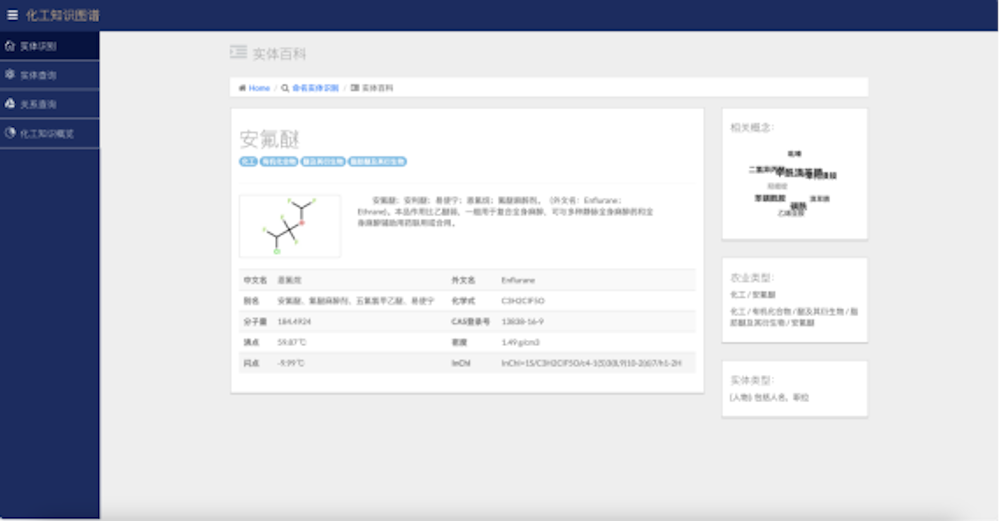
\includegraphics[height=2.20in,width=4.00in,viewport=0 0 240 130,clip]{Figures/KG_Chem-Enflurane.png}
\caption{\tiny 知识图谱的词条内容:~化合物\textrm{安氟醚}的有关知识}%(与文献\cite{EPJB33-47_2003}图1对比)
\label{Fig:KG_Chem-Enflurane}
\end{figure}
\end{frame}

%\frame
%{
%	\frametitle{化学-化工知识图谱的组成}
%\begin{figure}[h!]
%\centering
%\vskip -8pt
%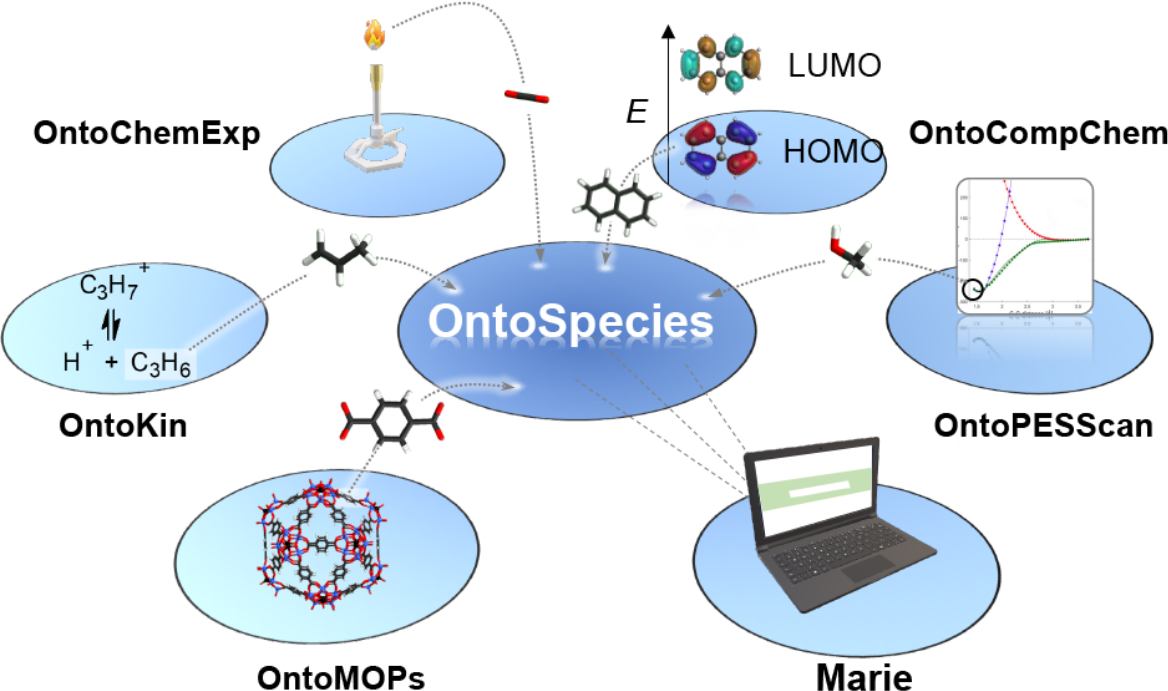
\includegraphics[height=2.45in,width=4.05in,viewport=0 0 1170 700,clip]{Figures/Connection-of-OntoSpecies-to-segments-of-KG.png}
%\caption{\tiny\textrm{Connection of OntoSpecies to other segments of TWA KG. cite from~\cite{ACR56-128_2023}}}%(与文献\cite{EPJB33-47_2003}图1对比)
%\label{Fig:OntoSpecies-to-segments-TWA}
%\end{figure}
%}
%
%\frame
%{
%	\frametitle{化学-化工知识图谱}
%	化学-化工知识图谱:~以化学物种(元素、化合物)为核心的\textcolor{cyan}{多个知识的\textrm{Ontology}组成}
%	\begin{itemize}
%		\item \textrm{OntoSpecites}:~主要纪录化学物种的知识,包括分子式、电荷、分子量和自旋多重度等
%		\item \textrm{OntoKin}:~表示反应机理的知识,纪录反应物、产物和反应过程的信息
%		\item \textrm{OntoCompChem}:~表示计算化学的信息的知识,计算信息的描述包括
%			\begin{itemize}
%				\item 计算对象:~单点计算、结构优化和频率计算
%				\item 计算使用的软件,{\fontsize{7.2pt}{5.2pt}\selectfont{如\textrm{Gaussian~16}}}
%				\item 计算中使用的方法,包括泛函和基组{\fontsize{7.2pt}{5.2pt}\selectfont{~如\textrm{B3LYP,~6-31G(d)}}}
%				\item 电荷与自旋极化
%			\end{itemize}
%		\item \textrm{OntoCompExp}:~表示化学实验信息的知识,包括各类化学实验条件
%	\end{itemize}
%}
%
%\frame
%{
%	\frametitle{\textrm{OntoSpecies}:~化学物种的描述}
%\begin{figure}[h!]
%\centering
%\vskip -8pt
%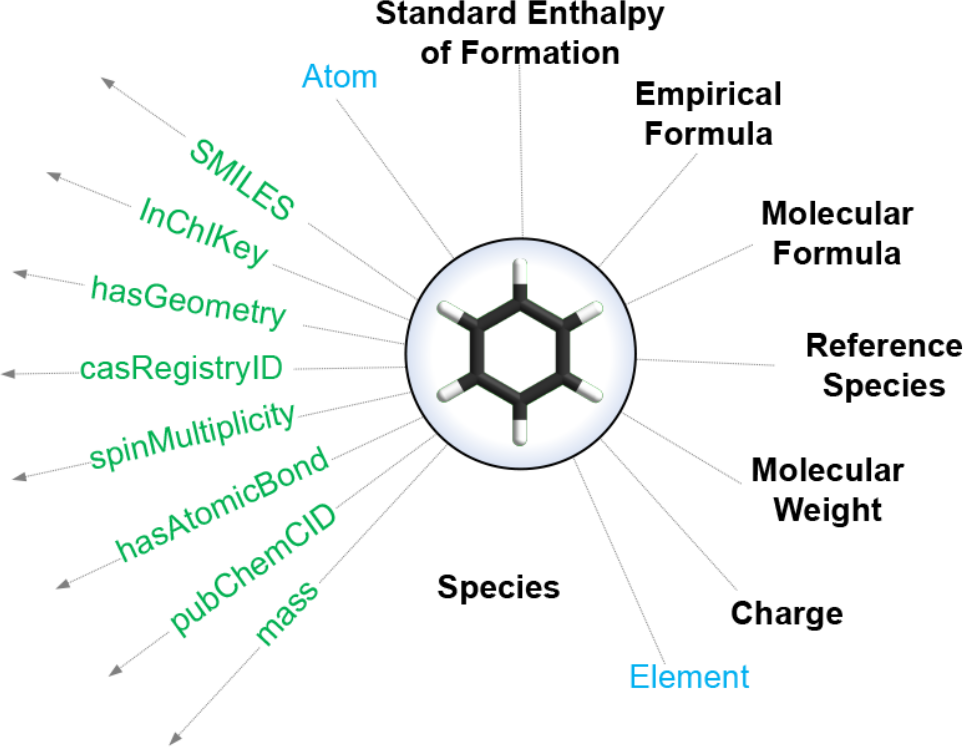
\includegraphics[height=2.40in,width=3.25in,viewport=0 0 990 750,clip]{Figures/Key_OntoSpecies-and-external_concepts.png}
%\caption{\tiny\textrm{Key OntoSpecies (black) and external (blue) concepts, along with a number of properties (green) used to describe chemical species in TWA KG. cite from~\cite{ACR56-128_2023}}}%(与文献\cite{EPJB33-47_2003}图1对比)
%\label{Fig:Key-OntoSpecies-and-external-concepts}
%\end{figure}
%}
%
%\frame
%{
%	\frametitle{\textrm{Agent}:~化学-化工知识图谱的组织工具}
%	\textrm{Agent}:~能够感知环境、进行决策和执行动作的智能处理软件
%	\begin{itemize}
%		\item \textrm{Agent}工作方式类似于人类代理:~能接收输入数据(如传感器信息、文本、图像等),通过分析和处理数据,理解环境和任务要求,并做出相应的决策和行动
%		\item 应用场景广泛,如自动驾驶车辆、智能机器人、语音助手等
%		\item \textrm{Agent}核心功能:~感知、推理和决策
%			\begin{itemize}
%				\item 感知:~通过传感器等方式获取环境信息的能力,例如通过摄像头获取图像或通过麦克风获取声音
%				\item 推理:~基于获取的信息进行逻辑推理和分析的能力,以了解环境和任务需求
%				\item 决策:~根据推理结果做出相应的决策,并执行相应的动作
%			\end{itemize}
%		\item 通过与环境的交互和反馈,\textrm{Agent}可以逐步改进性能和表现,实现好的任务执行能力\\
%		\item \textrm{Agent}设计和训练,需要结合机器学习和人工智能技术,如强化学习、深度学习等
%	\end{itemize}
%}
%
%\frame
%{
%	\frametitle{知识图谱组织示例}
%\begin{figure}[h!]
%\centering
%\vskip -8pt
%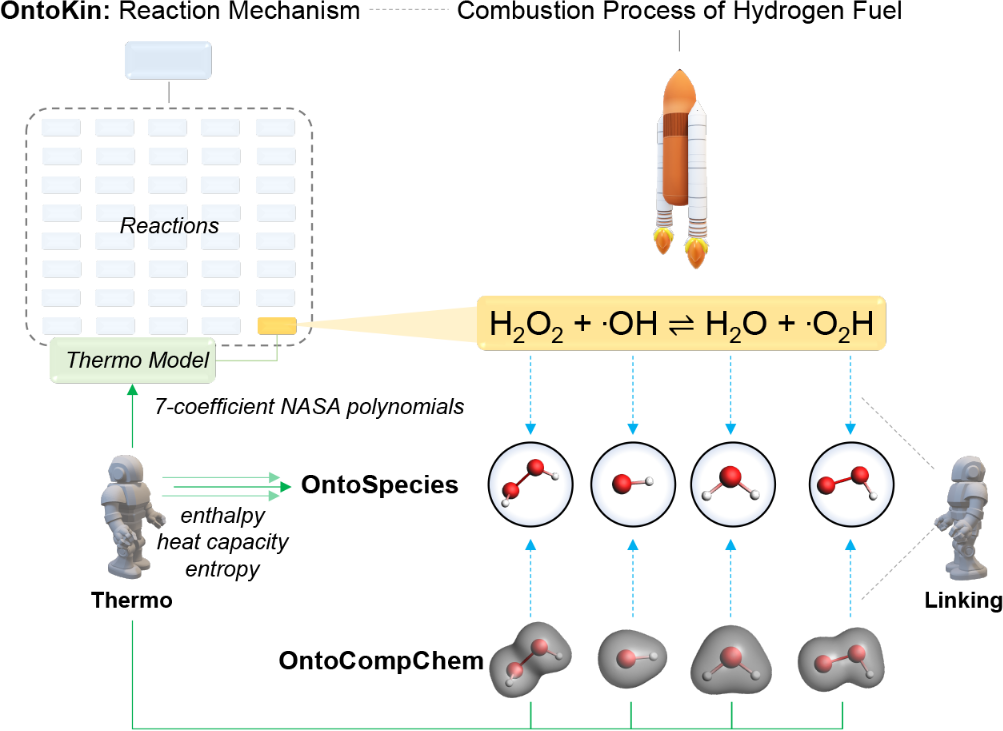
\includegraphics[height=2.70in,width=3.75in,viewport=0 0 1010 750,clip]{Figures/Automated-linking-between-OntoSepcies-Kin-CompChem.png}
%\caption{\tiny\textrm{Automated linking between OntoSpecies, OntoKin and OntoCompChem. cite from~\cite{ACR56-128_2023}}}%(与文献\cite{EPJB33-47_2003}图1对比)
%\label{Fig:Automated-linking-between-OntoSpecies-Kin-CompChem}
%\end{figure}
%}
%
%\frame
%{
%	\frametitle{知识图谱组织示例}
%\begin{figure}[h!]
%\centering
%\vskip -8pt
%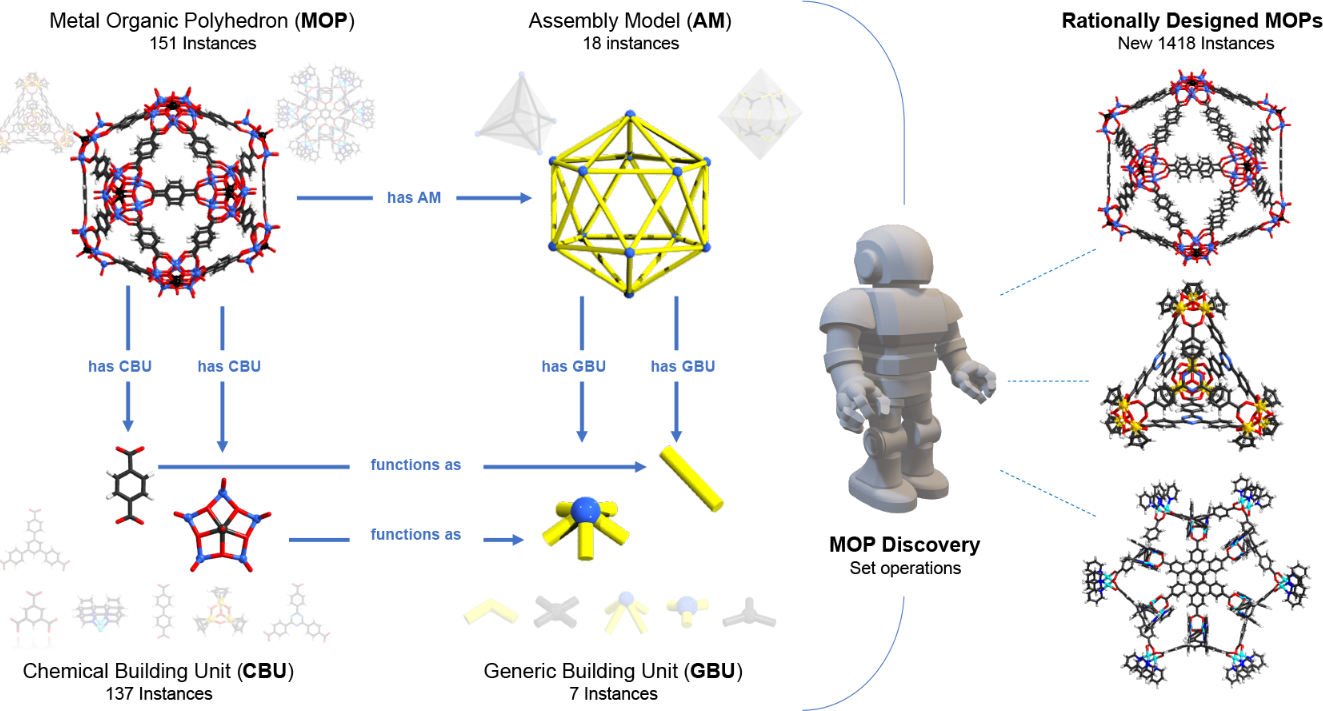
\includegraphics[height=2.20in,width=4.05in,viewport=0 0 1330 700,clip]{Figures/Key_concepts-in-OntoMOPs-and-designed-MOPs.png}
%\caption{\tiny\textrm{Key concepts in OntoMOPs (left) and examples of newly rationally designed MOPs (right). cite from~\cite{ACR56-128_2023}}}%(与文献\cite{EPJB33-47_2003}图1对比)
%\label{Fig:OntoMOPs-MOPs}
%\end{figure}
%}

%\begin{frame}
%	\frametitle{应用:~类石墨烯材料的稳定性优化预测}
%\begin{figure}[h!]
%\centering
%%\hskip -35pt
%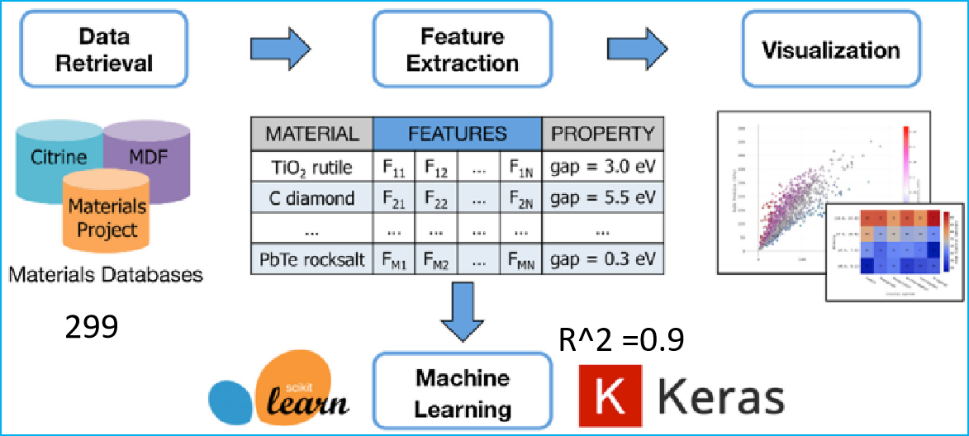
\includegraphics[height=1.55in]{Figures/MP_comp_BCC-5.png}
%%\caption{\fontsize{6.5pt}{4.5pt}\selectfont{面向多尺度材料智能计算平台}}%
%\label{MP_comp_BCC_5}
%\end{figure}
%{\fontsize{7.5pt}{5.5pt}\selectfont{
%	\begin{itemize}
%		\item 应用高通量建模软件构建潜在构型5600多种,利用\textrm{Materials~Projects}材料计算数据库提取竞争相数据
%		\item 通过热分解过程,组合化学反应式2000多组,筛选出热力学稳定的材料299种
%		\item 通过支持向量、高斯过程、随机深林、神经网络以及\textrm{adaboost}多种机器学习回归模型,利用13种常见特征参数对稳定性做了预测
%		\item 预测准确率达到94\%,节省计算成本高达70\%
%	\end{itemize}}}
%\end{frame}
%
%\begin{frame}
%	\frametitle{应用:~监督学习预测半导体材料带隙}
%\begin{figure}[h!]
%\centering
%\hspace*{-8pt}
%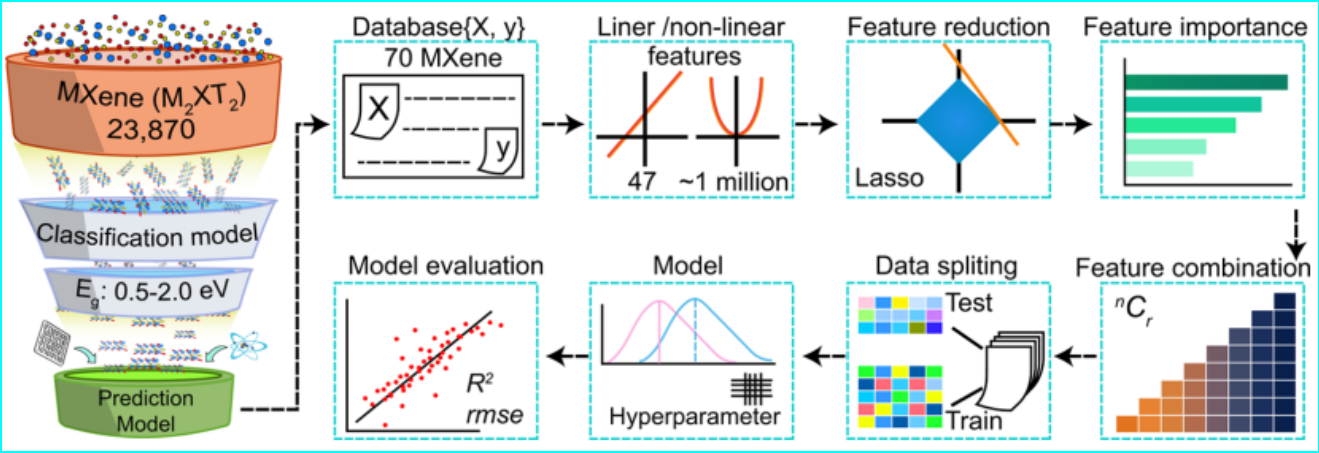
\includegraphics[height=1.45in]{Figures/MP_comp_BCC-6.png}
%%\caption{\fontsize{6.5pt}{4.5pt}\selectfont{面向多尺度材料智能计算平台}}%
%\label{MP_comp_BCC_6}
%\end{figure}
%{\fontsize{7.5pt}{5.5pt}\selectfont{
%	\begin{itemize}
%		\item 常规通行的材料模拟中带隙计算相当耗时
%		\item 利用%类石墨烯新能源
%	材料高通量智能计算与多目标机器学习集成研发平台,高通量自动化快速构建类石墨烯材料结构23870种,并构建数据库结合\textrm{KRR}、\textrm{SVR}、\textrm{GPR}、\textrm{Bagging}机器学习回归模型进行训练预测
%		\item \textrm{GPR}方法预测准确性达到了97\%,可以节省计算成本90\%多
%	\end{itemize}}}
%\end{frame}

%\begin{frame}[allowframebreaks]
%	\frametitle{主要合作与推广应用}
%		中科合成油(合作)
%	\begin{itemize}
%	 \setlength{\itemsep}{30pt}
%	\item 化学-化工知识图谱的建设
%\begin{figure}[h!]
%\centering
%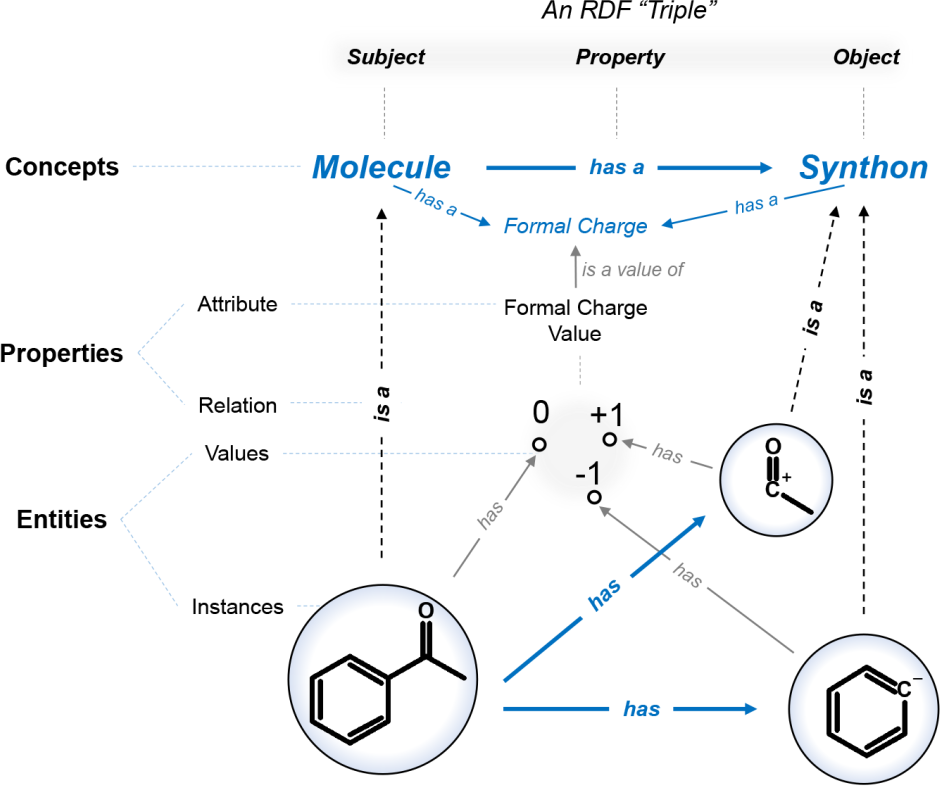
\includegraphics[height=1.50in,width=1.75in,viewport=0 0 950 790,clip]{Figures/Mapping-the-relationship-between-molecule-and-synthon.png}
%\hspace{5pt}
%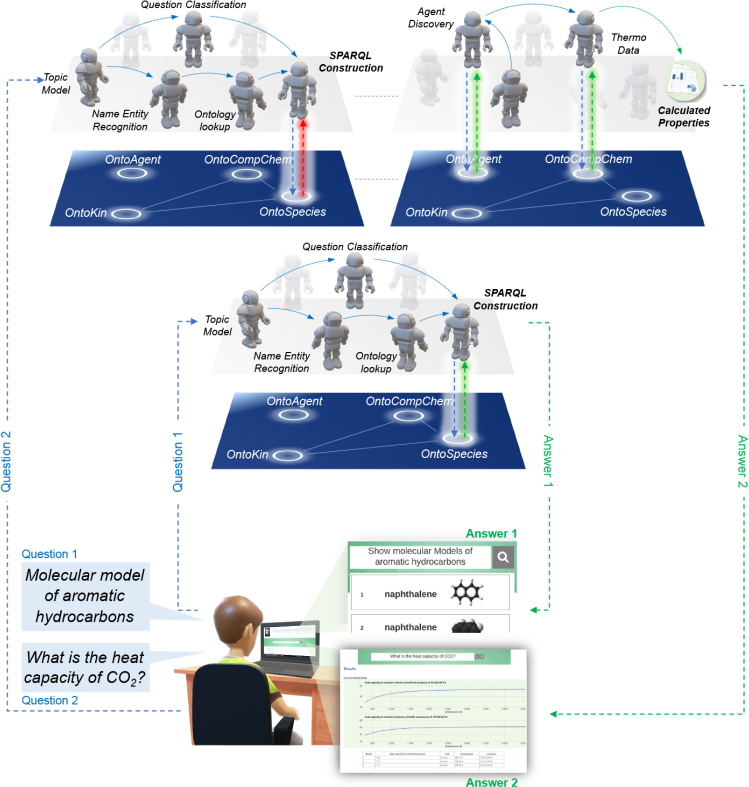
\includegraphics[height=1.50in,width=1.55in,viewport=0 0 750 790,clip]{Figures/TWA-KG-Marie.png}
%%\caption{\small\textrm{Mapping the relationship molecule (chemical) and synthon (abstract) concepts and illustrating them with instrances. cite from~\cite{ACR56-128_2023}}}%(与文献\cite{EPJB33-47_2003}图1对比)
%\label{Fig:Mapping-relationship-molecule-synthon}
%\end{figure}
%	\begin{itemize}
%{\fontsize{7.5pt}{5.5pt}\selectfont{
%		\item 以化合物为核心,借助语义网\textrm{(Semantic Web)},组织、表示和存储化学-化工和领域特定类型的知识
%		\item 构建拥有学习和推理能力,具备初级的创造知识的能力}}
%	\end{itemize}
%	\item 问-答式煤化工智能模型建设
%\begin{figure}[h!]
%\centering
%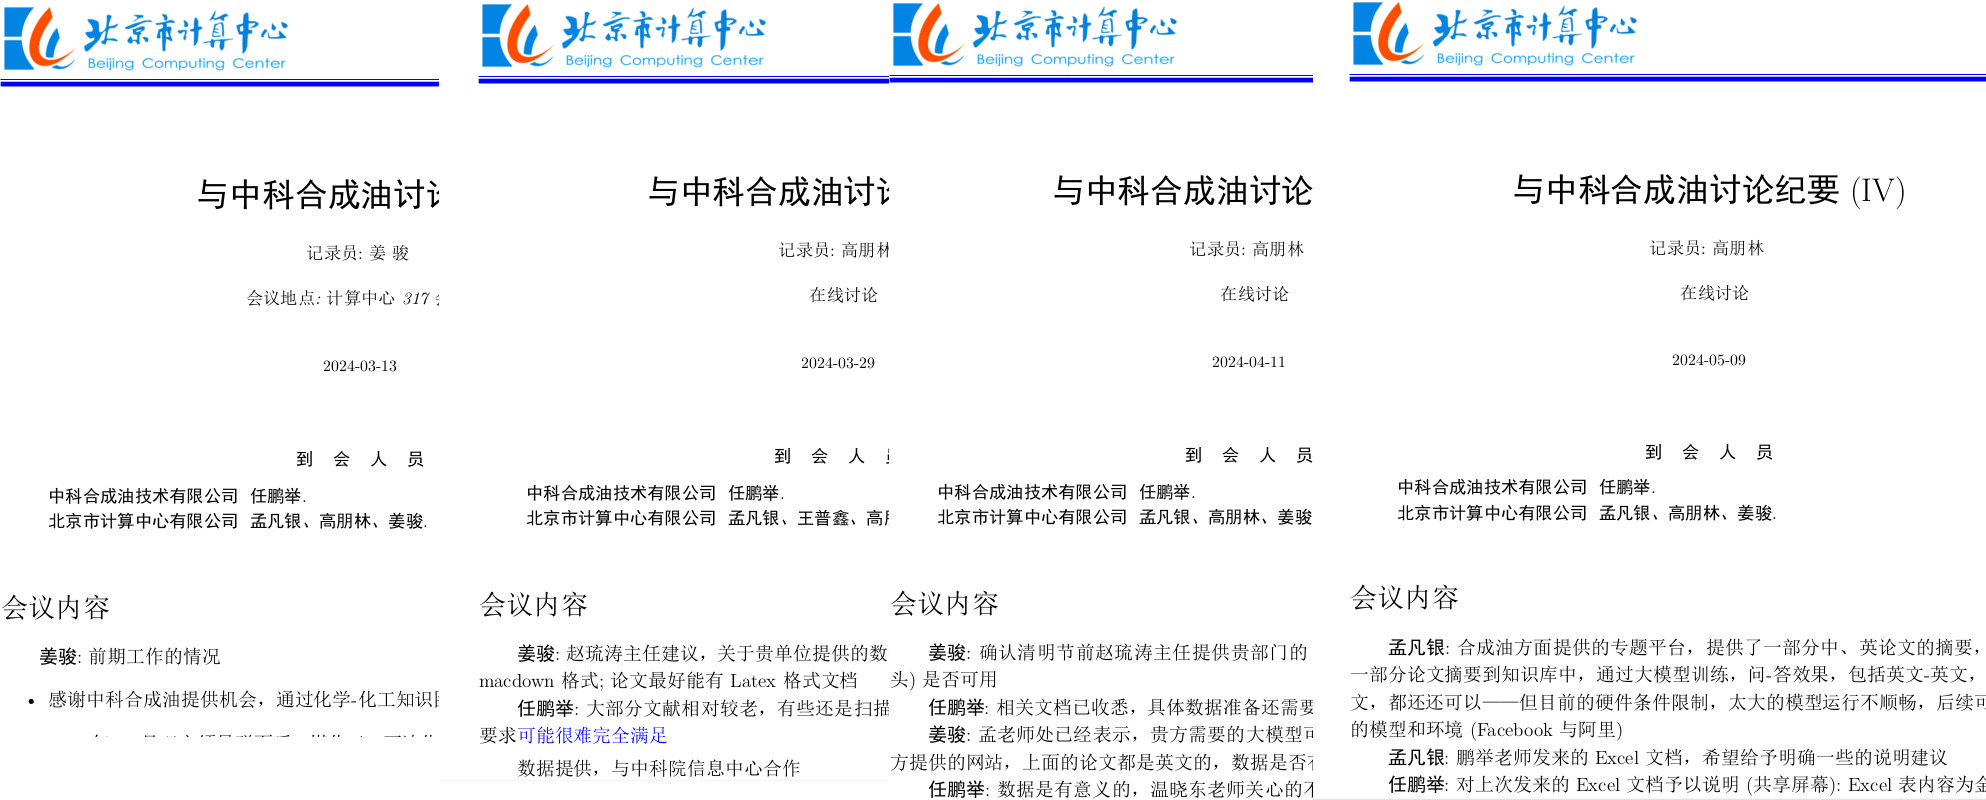
\includegraphics[height=1.40in,width=3.50in,viewport=0 0 1986 800,clip]{Figures/MeetingRecord_SCTC-BCC.png}
%\label{Fig:Meeting_Record}
%\end{figure}
%\begin{itemize}
%	\item 面向人工智能的全方位转型:\\
%		面向碳基础材料、发挥人工智能的作用
%	\item 大模型加持专业知识
%\end{itemize}
%	\end{itemize}
%\textcolor{purple}{目标:}~智能实验室-智能科学家
%\end{frame}
%
%\begin{frame}
%	\frametitle{数据驱动的材料研发:~应用前景}
%	\begin{enumerate}
%	 \setlength{\itemsep}{20pt}
%	 \item 航空发动机材料:~\textcolor{blue}{镍基单晶高温合金材料}\\
%	合金组分优化与强化功能提升
%
%\item 煤化工催化材料:~\textcolor{blue}{新型铁触媒材料}\\
%	反应活化性能提升与化学平衡的移动
%
%		\item 稀土功能材料:~\textcolor{blue}{钕铁硼永磁材料},\textcolor{blue}{稀土发光材料}\\
%	3\textit{d}-4\textit{f} 电子相互作用机制的认知
%
%	\end{enumerate}
%
%	\textcolor{magenta}{材料组分趋于复杂、材料机理认知趋于微观、材料与数据趋于膨胀}
%%\begin{figure}[h!]
%%\vspace*{-0.20in}
%%\centering
%%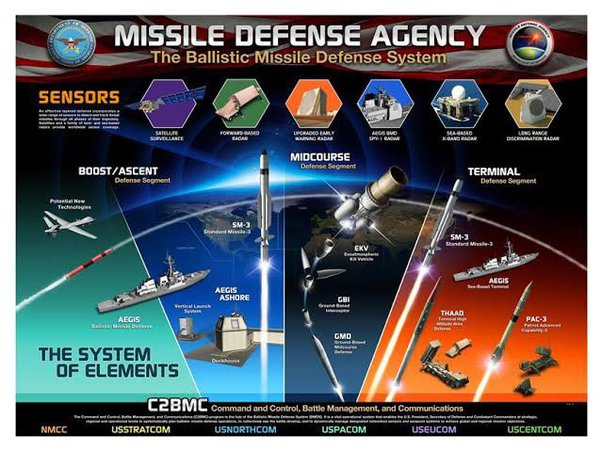
\includegraphics[height=2.90in,width=3.70in]{Figures/Main-qimg.jpeg}
%%\label{BMDS}
%%\end{figure}
%\end{frame}
%------------------------------------------------------------------------Reference----------------------------------------------------------------------------------------------
%		\frame[allowframebreaks]
%{
%\frametitle{主要参考文献}
%\begin{thebibliography}{99}
%{\tiny
%	\bibitem{PR136-B864_1964}\textrm{P. Hohenberg and W. Kohn, \textit{Phys. Rev.} \textbf{136} (1964), B864}
%	\bibitem{PR140-A1133_1965}\textrm{W. Kohn and L.J. Sham, \textit{Phys. Rev.} \textbf{140} (1965), A1133}
%	\bibitem{PRB50-17953_1994}\textrm{P. E. Bl\"ochl. \textit{Phys. Rev.} B, \textbf{50} (1994), 17953}
%	\bibitem{PRB59-1758_1999}\textrm{G. Kresse and D. Joubert \textit{Phys. Rev.} B, \textbf{59} (1999), 1758}
%	\bibitem{Elect_Stru}\textrm{Richard. M. Martin. \textit{Electronic Structure: Basic Theory and Practical Methods} (Cambridge University Press, Cambridge, England, 2004)}
%        \bibitem{Singh}\textrm{D. J. Singh. \textit{Plane Wave, PseudoPotential and the LAPW method} (Kluwer Academic, Boston,USA, 1994)}					%
%}
%\end{thebibliography}
%%\nocite*{}
%}

\appendix
\section{\rm{AI}大模型}
\begin{frame}
	\frametitle{零样本\textrm{LLM}的知识图谱构建}
\begin{figure}[h!]
\centering
\vskip -8pt
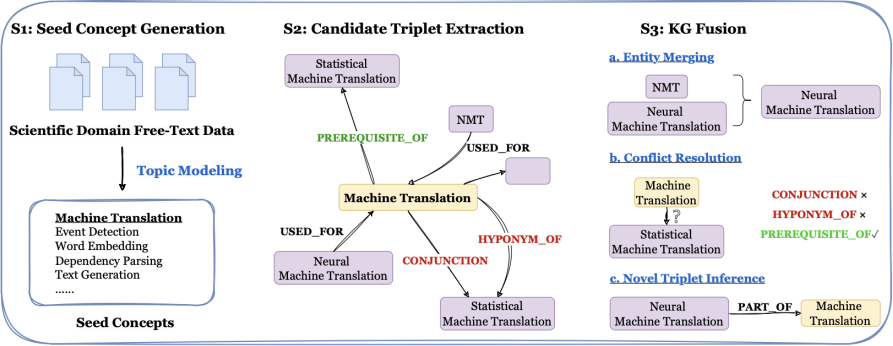
\includegraphics[height=2.2in,width=3.90in,viewport=0 0 215 90,clip]{Figures/KG_Chem-KG-LLM.png}
\caption{\tiny\textrm{文献出处:~\url{https://arxiv.org/abs/2410.17600}}}%(与文献\cite{EPJB33-47_2003}图1对比)
\label{Fig:KG_Chem-LLM_KG}
\end{figure}
\end{frame}

\begin{frame}
	\frametitle{大模型与知识图谱的关系}
\begin{figure}[h!]
\centering
\vskip -8pt
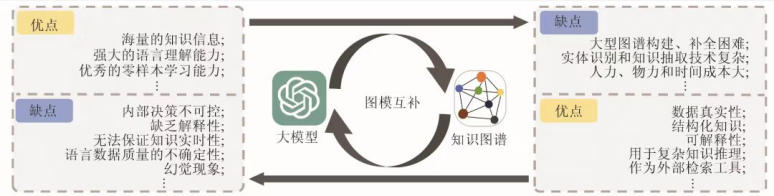
\includegraphics[height=1.2in,width=3.90in,viewport=3 0 185 60,clip]{Figures/KG_Chem-LLM.png}
\caption{\tiny\textrm{大模型与知识图谱的互补关系}}%(与文献\cite{EPJB33-47_2003}图1对比)
\label{Fig:KG_Chem-LLM}
\end{figure}
\begin{itemize}
	\item {\fontsize{7.2pt}{6.2pt}\selectfont{知识图谱对大模型的增强:~为大模型提供真实可靠的知识,减轻大模型产生幻觉的问题,提供解释和推理知识的手段,探究大模型内部复杂的工作步骤和推理过程}}%,还可以作为外部检索工具,帮助大模型解决公平、隐私和安全等问题
	\item {\fontsize{7.2pt}{6.2pt}\selectfont{大模型对知识图谱的增强:大模型在零样本和少样本的训练中,能够应对知识图谱构建、补全、推理和问答等各种挑战}}%。例如,大模型可以利用零样本或少样本学习的信息提取能力,从文本或其他数据源中完成实体抽取和关系抽取任务,节约数据标注的时间和成本;还可以作为额外知识库提取可信知识,完成知识图谱的补全。
\end{itemize}
\end{frame}

\subsection{通用语义大模型的搭建}
\begin{frame}
	\frametitle{知识问答大模型的搭建}
\begin{figure}[h!]
\centering
\vskip -8pt
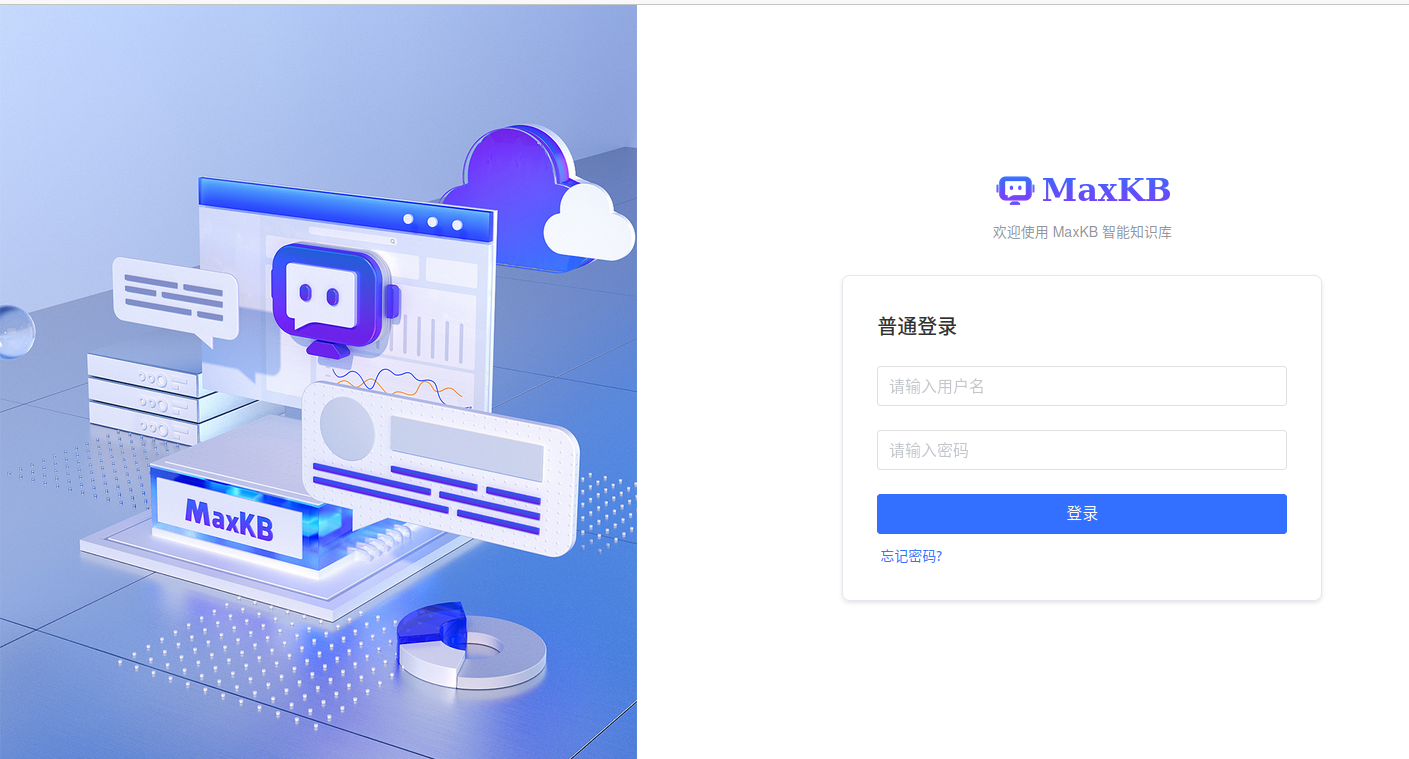
\includegraphics[height=1.90in,width=3.75in,viewport=0 0 1409 750,clip]{Figures/MaxKB_login.png}
\caption{\tiny\textrm{The login of MaxKB}}%(与文献\cite{EPJB33-47_2003}图1对比)
\label{Fig:MaxKB_login}
\end{figure}
{\fontsize{7.5pt}{6.0pt}\selectfont{化学-化工知识助手基于通用的\textrm{MaxKB}大模型知识问答系统搭建 (当前通用模型大小约\textrm{13TB}),主要通过对中科合成油提供的数据(主要是文献,约\textrm{500}篇)的学习,训练面向煤化工研究的专业知识问-答模型}}
\end{frame}

\begin{frame}
	\frametitle{知识问答大模型的搭建}
\begin{figure}[h!]
\centering
\vskip -8pt
\includegraphics[height=2.2in,width=3.90in,viewport=3 0 1848 1041,clip]{Figures/MaxKB_Creat-APP.png}
\caption{\tiny\textrm{The Configuration of MaxKB}}%(与文献\cite{EPJB33-47_2003}图1对比)
\label{Fig:MaxKB_Creat-APP}
\end{figure}
\end{frame}

\begin{frame}
	\frametitle{知识问答大模型的搭建}
\begin{figure}[h!]
\centering
\vskip -8pt
\includegraphics[height=2.20in,width=3.90in,viewport=0 0 1850 1041,clip]{Figures/MaxKB_Chose-Model.png}
\caption{\tiny\textrm{The Configuration of MaxKB}}%(与文献\cite{EPJB33-47_2003}图1对比)
\label{Fig:MaxKB_Chose-Model}
\end{figure}
\end{frame}

\begin{frame}
	\frametitle{知识问答大模型的搭建}
\begin{figure}[h!]
\centering
\vskip -8pt
\includegraphics[height=0.80in,width=3.90in,viewport=0 650 1850 1054,clip]{Figures/MaxKB_NewDatabase.png}
\includegraphics[height=1.80in,width=3.90in,viewport=0 0 1850 880,clip]{Figures/MaxKB_Database.png}
\caption{\tiny\textrm{Uploading a New File to the Database}}%(与文献\cite{EPJB33-47_2003}图1对比)
\label{Fig:MaxKB_Database}
\end{figure}
\end{frame}

\subsection{化学-化工知识问答}
\begin{frame}
	\frametitle{化学-化工知识的大模型数据}	
\begin{figure}[h!]
\centering
%\vskip -8pt
\includegraphics[height=2.10in,width=4.00in,viewport=0 0 1149 636,clip]{Figures/MaxKB_Info-1.png}
\caption{\tiny\textrm{Data uploaded for MaxKB}}%(与文献\cite{EPJB33-47_2003}图1对比)
\label{Fig:MaxKB_Data-1}
\end{figure}
\end{frame}

\begin{frame}
	\frametitle{化学-化工知识的大模型数据}	
\begin{figure}[h!]
\centering
%\vskip -8pt
\includegraphics[height=1.90in,width=4.00in,viewport=0 0 1456 647,clip]{Figures/MaxKB_Info-2.png}
\caption{\tiny\textrm{Data uploaded for MaxKB}}%(与文献\cite{EPJB33-47_2003}图1对比)
\label{Fig:MaxKB_Data-2}
\end{figure}
\end{frame}

\begin{frame}
	\frametitle{化学-化工知识问答:~示例}	
\begin{figure}[h!]
\centering
%\vskip -8pt
\includegraphics[height=2.30in,width=4.00in,viewport=0 0 1528 875,clip]{Figures/MaxKB_Chem.png}
\caption{\tiny\textrm{\url{http://123.59.0.69:8080/ui/chat/f6385eb7c6c8a618}}}%(与文献\cite{EPJB33-47_2003}图1对比)
\label{Fig:MaxKB_Chem}
\end{figure}
\end{frame}

\begin{frame}
	\frametitle{化学-化工知识问答:~示例}	
\begin{figure}[h!]
\centering
\vskip -8pt
\includegraphics[height=1.40in,width=3.30in,viewport=0 0 978 447,clip]{Figures/Allma_MaxKB-1.png}
\includegraphics[height=1.30in,width=3.30in,viewport=0 342 924 759,clip]{Figures/Allma_MaxKB-2.png}
%\includegraphics[height=2.60in,width=3.70in,viewport=0 0 924 759,clip]{Figures/Allma_MaxKB-2.png}
\caption{\tiny\textrm{Chemical-Chemistry Chat-Model}}%(与文献\cite{EPJB33-47_2003}图1对比)
\label{Fig:MaxKB_Chat-Model-2}
\end{figure}
\end{frame}
%
\frame
{
	\frametitle{化学-化工知识组织和生成的一些建议}
	\textcolor{red}{数据是形成知识的基础}:~\\
	面向科学问题,软件对关联数据的组织、表达、逻辑认知和理解表达能力有待提升,需要专业人力支持\\
	当数据量较少时,软件对科学数据的学习、挖掘和完善能力,与预期有一定的距离
	\begin{itemize}
		\item 化学-化工涉及知识点广泛,很难用很少的几个知识点简单地涵盖,化学-化工知识生态还有赖组织和构建
%	建议参照上述化学-化工知识图谱方案,
%		\item 以化学物种数据为核心知识
%		\item 化学实验、化学计算知识的储备为桥梁
%		\item 化学反应-实验、计算-物种的数据关联为目标
%		\item 扩展各\textrm{Ontology}间数据分析、传递的\textrm{Agent}功能
%		\item 通过\textrm{Ontology}-\textrm{Agent}数据迭代直至自洽
%		\item 通过复杂计算和逻辑推理,产生新的物种属性描述或新的知识
		\item 将通用大语言模型\textrm{(Large Language Model)}训练成为适合化学-化工场景的应用,对数据的完整性有很大的依赖
	\end{itemize}
	\textcolor{magenta}{近期目标}:~面向以分子或材料为中心的知识,不断积累、完善知识点的内涵,改进和提升对知识内在逻辑的准确描述

\textcolor{magenta}{远期目标}:~建设完整的化学-化工(重点是煤化工)知识的生态系统,通过化学知识空间的探索,有效地发现更多的新化学知识
}
